\documentclass[a4paper,12pt]{article}


\usepackage{relsize}
\usepackage[margin=3cm]{geometry} %Definiere Rand
\usepackage{graphicx} % Zum Einbinden von Bildern
\usepackage[english]{babel} % Direkte Eingabe von Umlauten
%\UseRawInputEncoding
\usepackage[T1]{fontenc}  % Direkte Eingabe von Umlauten
\usepackage{pgfplots} % Zum Einfuegen von Plots
\pgfplotsset{compat=1.14} % Damit wird beim Plotten keinen Error bekommen
\usepackage[section]{placeins} %Damit Bilder in der Section bleiben
\usepackage{amsmath} % Standard fuer mathematische Ausdruecke
\usepackage{amssymb} % Weitere Symbole
\usepackage{mathtools} % Fuer weitere mathematische Ausdruecke
\usepackage{dsfont}
\usepackage[font=small,labelfont=bf]{caption} % Kleinerer Text bei Captions
\usepackage{tabu} % Anderes Tabellenenvironment, wird am Ende fuer die Namen verwendet
\usepackage{subcaption} % Side-by-side figures with minipage
\usepackage{url} % Damit man urls zitieren kann
\usepackage[autostyle=true,german=quotes]{csquotes} % Damit Zitieren leichter ist; Bsp: \enquote{nur}
\usepackage[nottoc,numbib]{tocbibind} % Damit die Referenzen im Inhaltsverzeichnis erscheinen
\usepackage{standalone} % Zum Outsourcen von Plots
\usepackage{setspace} % Damit die naechsten funktionieren
\renewcommand{\topfraction}{0.85} % Let top 85% of a page contain a figure
\renewcommand{\textfraction}{0.1} % Default amount of minimum text on page (Set to 10%)
\renewcommand{\floatpagefraction}{0.75} % Only place figures by themselves if they take up more than 75% of the page
%
\usepackage{threeparttable, tablefootnote}
\usepackage[colorlinks,urlcolor=black,allcolors=.]{hyperref} % For hyperlinks to be clickable
\usepackage{listings} % For embedding code into the document
\usepackage{bm} % For bold italic letters in math mode, shorter than \boldsymbol
\usepackage{amsthm} % For theorems, definitions, examples, etc.
\usepackage{empheq} % For alignment inside cases
\pgfplotsset{compat=1.16} % To avoid tikz errors
\usepackage{tcolorbox} % For boxes around text
\usepackage{enumitem} % For enumerate and itemize, custom separations
\usepackage{bbold} % For \mathbb{1}
\usepackage{xcolor, soul} % For text with color background
\definecolor{lightlightgray}{RGB}{224,224,224}
\sethlcolor{lightlightgray} % Color background color
\usepackage{algorithm} % For algorithm environment
\usepackage{algpseudocode} % For pseudocode
\newcommand{\Statein}{\State \hspace{\algorithmicindent}}

% begin vertical rule patch for algorithmicx (http://tex.stackexchange.com/questions/144840/vertical-loop-block-lines-in-algorithmicx-with-noend-option)
\makeatletter
% start with some helper code
% This is the vertical rule that is inserted
\newcommand*{\algrule}[1][\algorithmicindent]{\makebox[#1][l]{\hspace*{.5em}\vrule height .75\baselineskip depth .25\baselineskip}}%

\newcount\ALG@printindent@tempcnta
\def\ALG@printindent{%
    \ifnum \theALG@nested>0% is there anything to print
        \ifx\ALG@text\ALG@x@notext% is this an end group without any text?
            % do nothing
            \addvspace{-3pt}% FUDGE for cases where no text is shown, to make the rules line up
        \else
            \unskip
            % draw a rule for each indent level
            \ALG@printindent@tempcnta=1
            \loop
                \algrule[\csname ALG@ind@\the\ALG@printindent@tempcnta\endcsname]%
                \advance \ALG@printindent@tempcnta 1
            \ifnum \ALG@printindent@tempcnta<\numexpr\theALG@nested+1\relax% can't do <=, so add one to RHS and use < instead
            \repeat
        \fi
    \fi
    }%
\usepackage{etoolbox}
% the following line injects our new indent handling code in place of the default spacing
\patchcmd{\ALG@doentity}{\noindent\hskip\ALG@tlm}{\ALG@printindent}{}{\errmessage{failed to patch}}
\makeatother
% end vertical rule patch for algorithmicx

% Adds vertical lines to algorithm loops, for better visibility
\makeatletter
\newcommand{\algmargin}{\the\ALG@thistlm}
\makeatother
\algnewcommand{\parState}[1]{\State%
  \parbox[t]{\dimexpr\linewidth-\algmargin}{\strut #1\strut}}

% Putting this here because in the standalone it does not work
% Wasted a half day on this!
\usetikzlibrary{shapes.geometric}
\usetikzlibrary{arrows.meta, trees}
\usetikzlibrary{arrows,shapes}
\newcommand{\mySize}{\small}
\newcommand{\nodeSep}{0.75}


\begin{document}
\usetikzlibrary{patterns}

%
    \title{Tuning learning of circuit-based classifiers\\
    \vspace{2em}
    Master's Thesis\\
    \vspace{2em}
    JKU Linz\\
    \vspace{1.5em}
    from}

    \author{
 	\LARGE Bernhard Gstrein\\
 	\vspace{.5em} \\
 	Supervisors:\\
 	Martina Seidl\\
 	Armin Biere\\
 	\vspace{1em}
	}
    
\date{Linz, 2022}

\maketitle
   
\begin{abstract}
\noindent Neural networks have proven to work remarkably well and are prevalent in our everyday lives. Two major concerns, however, are computational cost while training and during inference and the model size. To address these concerns, we remind ourselves that on a computer, everything is represented by 0s and 1s. Working at low level could be a step towards efficiency in terms of compute and disk space. This thesis explores the questions whether building a predictive system that natively works with binary values is possible and in the case that this is true, whether there are any advantages compared to gradient descent with backpropagation at its core.
\end{abstract}
   
\newpage
   
\tableofcontents
 
\newpage
    

\section{Introduction}
Neural networks trained using gradient descent work remarkably well which is the reason for their universal use. Small neural networks have their place, but it is the large neural networks that perform complex tasks, such as translation, object recognition or autonomous driving. The more parameters, the more compute during training and inference is required and the environmental impact is a concern \cite{bib:schwartz2020green}. A cumbersome aspect of neural network-powered AI is that many models are stored on a remote server and data has to be sent over the internet. The requirement of a constant and (in most cases) fast internet connection is a serious inhibitor to applying neural networks in practice. Without being able to transmit all of its input data to a server, devices with small computing power and little storage, such as autonomous lawn mowers, intelligent cameras, smart sensors, etc, have no means to run a big neural netork.

\subsection{Approach}
We know that a neural network basically is just a sequence of matrix operations; our input is transformed and we obtain a quantity of our interest which could be a probability, a number, a synthesized image, etc. We also know that a computer works with binary values, i.e., 0s and 1s. In the end, a representation of a neural network is a sequence of 0s and 1s, so is the input to the neural network and the output, which raises the question if we can \textit{directly} work with binary values, skipping layers of abstraction. Perhaps such a scheme would be more environmentally friendly since it does not require floating point operations. A small binary model, i.e., circuit,  that requires little compute and disk space might be a good step towards making AI more prevalent and reducing costs. Extensive research already exists to make existing neural architectures smaller to apply them at edge devices \cite{bib:liu2021bringing} which also includes binary architectures. However, most existing approaches to reduce model size into binary start with regular models and gradually transfer them to binary. We already start at binary.

\subsection{Outline}
Our questions of interest are summarized in the list below. We address (\ref{enum:build}) by looking at 2 schemes to build network-like architectures, where the former is described in a paper \cite{bib:chatterjee2018learning} and the latter we invent ourselves. We evaluate training and testing accuracies of each architecture (\ref{enum:performance}), calculate the size they take up on disk (\ref{enum:disk_space}) and discuss the computational power required to deploy these models (\ref{enum:efficiency}). The sub-items of (\ref{enum:practical}) we discuss to our best knowledge, but might only give a hint what is possible given there is room for improvement (\ref{enum:room}).

\begin{enumerate}
  \item \label{enum:build} Is it possible to build a predictive system that works entirely in binary?
  \item \label{enum:practical} Is it practical to build a predictive system working in binary? Concretely, does a predictive system working with binary values...
    \begin{enumerate}
      \item \label{enum:performance} ...have a good performance in terms of accuracy?
      \item \label{enum:disk_space} ...take up less space on disk?
      \item \label{enum:efficiency} ...have a good performance in terms of computational efficiency?
    \end{enumerate}
  \item \label{enum:room} Is there room for improvement?
\end{enumerate}

\noindent Lastly, we would like to already give away what we achieved in this thesis. Figure~\ref{fig:model_performance} visualizes testing accuracies and size for different models. The more a point lies to the top and to the left, the better. The meaning of the model names we will introduce throughout this thesis. We took an existing approach of binary model from \cite{bib:chatterjee2018learning}, visible as $\color{green} \oplus$ in Figure~\ref{fig:model_performance}, and were able to improve accuracy and reduce size, visible as $\color{violet} \bigtriangleup$ in Figure~\ref{fig:model_performance}. On the lower-left corner we can see another binary model that we built, the \enquote{AIG}. It is the weakest model in terms of accuracy in Figure~\ref{fig:model_performance}, however, it is extremely small (just 68 Bytes) and easily translatable to a circuit on hardware, making this model a very good candidate for implementing on small electronic devices, also called \enquote{edge devices}.

\begin{figure}[!htb]
    \centering
    \includestandalone[]{standalone/lut/model_performance}
    \caption{Testing accuracy on the dataset \enquote{Binary-MNIST} and size for various models. The $x$-axis that represents the size has a logarithmic scale. The underlying data that was used to generate this plot can be seen in Table~\ref{tab:ml_algos_on_bmnist}. Our main contributions are $\color{violet} \bigtriangleup$, a binary model with improved accuracy and reduced sized compared to an existing approach $\color{green} \oplus$ and $\otimes$, a model that is extremely small and fast, albeit with lower accuracy.}
\label{fig:model_performance}
\end{figure}
\FloatBarrier

\section{Preliminaries}

In this section, we will give an overview of what neural networks are and how they are constructed. In general, we give the neural network a $d$-dimensional vector $\bm{x}$ (we denote vectors with variables in bold) as input and as output we obtain either a single number or another vector. The output is the \textit{prediction} of the neural network given the input $\bm{x}$. A few examples of predicted quantities given some input could be the price of a house given various information about it (e.g., age, size, location, etc.), the probability of a dark skin area being a melanoma given a picture of it or a Japanese translation given a German sentence. A neural network arrives at the prediction by \textit{transforming} the input. Concretely, matrix operations are being performed. As a simple example, consider input $\bm{x} \in \mathds{R}^{4 \times 1}$ and \enquote{weights} $\bm{w} \in \mathds{R}^{4 \times 1}$. The operation $\bm{w}^\top \cdot \bm{x} = \hat{y}$ yields a single number, the predicted quantity. The symbol $\cdot$ denotes the matrix product and the symbol $\hat{}$ denotes any variable below it is a prediction. Writing it out:

\begin{align} \label{eq:first_network}
    x_0 w_0 + x_1 w_1 + x_2 w_2 + x_3 w _3 = \hat{y}.
\end{align} If the weights have more than one column, e.g., if $\bm{W} \in \mathds{R}^{4 \times 3}$, then the operation $\bm{W}^\top \cdot \bm{x} = \hat{\bm{y}}$ yields a three-dimensional vector:

\begin{align} \label{eq:second_network}
    \begin{split}
        x_0 w_{00} + x_1 w_{10} + x_2 w_{20} + x_3 + w_{30} & = \hat{y}_0, \\
        x_0 w_{01} + x_1 w_{11} + x_2 w_{21} + x_3 + w_{31} & = \hat{y}_1, \\
        x_0 w_{02} + x_1 w_{12} + x_2 w_{22} + x_3 + w_{32} & = \hat{y}_2.
    \end{split}
\end{align}We can visualize the aforementioned matrix calculations using nodes and arrows, visible in Figure~\ref{fig:first_second_network}. The nodes represent individual entries of the respective vectors and the arrows multiplication with the weights. In Figure~\ref{fig:second_network}, we omitted writing the weights on the arrows for better visibility.


\begin{figure}[!htb]
    \centering
    \begin{subfigure}{0.4\textwidth}
      \centering
    \includestandalone[]{standalone/intro/first_network}
      \caption{Scalar output.}
      \label{fig:first_network}
  \end{subfigure}
  \begin{subfigure}{0.4\textwidth}
      \centering
    \includestandalone[]{standalone/intro/second_network}
      \caption{Vectorial output.}
      \label{fig:second_network}
  \end{subfigure}
  \caption{Matrix operations $\bm{w}^\top \cdot \bm{x} = \hat{y}$, $\bm{x} \in \mathds{R}^{4 \times 1}$, $\bm{w} \in \mathds{R}^{4 \times 1}$ in (\subref{fig:first_network}) and $\bm{W}^\top \cdot \bm{x} = \hat{\bm{y}}$, $\bm{x} \in \mathds{R}^{4 \times 1}$, $\bm{W} \in \mathds{R}^{4 \times 3}$ in (\subref{fig:second_network}) visualized. Each node is a scalar and an arrow protruding from it denotes the scalar is multiplied with a weight.}
\label{fig:first_second_network}
\end{figure}
\FloatBarrier

\noindent The calculations performed in Equation~\ref{eq:first_network} and Equation~\ref{eq:second_network} deliver a predicted quantity, however hardly any scholar would call them neural networks. Looking at following equation, we can be confident in stating it is a neural network:

\begin{align} \label{eq:third_network}
    \bm{W}^{[3]\top} \cdot \underbrace{h \big( \bm{W}^{[2]\top} \cdot \underbrace{h \big( \bm{W}^{[1]\top} \cdot \bm{x} \big)}_{\bm{a}^{[1]}} \big)}_{\bm{a}^{[2]}} = \hat{y},
\end{align}where $\bm{x} \in \mathds{R}^{4 \times 1}$, $\bm{W}^{[1]} \in \mathds{R}^{4 \times 5}$, $\bm{W}^{[2]} \in \mathds{R}^{5 \times 3}$, $\bm{W}^{[3]} \in \mathds{R}^{3 \times 1}$ and $h$ is an element-wise non-linear function. The intermediate results $\bm{a}^{[1]}$ and $\bm{a}^{[2]}$ are commonly called \enquote{activations}. Numbers in brackets are used to differentiate between variables and otherwise have no effect mathematically. Visualizing Equation~\ref{eq:third_network}, we obtain a graph structure as in Figure~\ref{fig:third_network}. We can see that the activations (i.e., intermediate results) are also represented using nodes. An array of nodes forming one activation vector we refer to as \enquote{hidden layer}.

\begin{figure}[!htb]
    \centering
    \includestandalone[]{standalone/intro/third_network}
    \caption{Equation~\ref{eq:third_network} visualized, a small neural network. The nodes between input and output represent intermediate results and are called \enquote{activations}. An array of nodes forming one activation vector we refer to as \enquote{hidden layer}.}
\label{fig:third_network}
\end{figure}
\FloatBarrier

\noindent When we refer to the \enquote{architecture} of a neural network, we mean the number of weight matrices, shape of weight matrices (i.e., how many rows and columns they have), types of activation functions and so on. The neural network depicted in Figure~\ref{fig:third_network} is small and simple, but enough for the sake of explaining. A good overview of different neural architectures can be found in \cite{bib:leijnen2020neural}. In case the reader wants to refresh their knowledge about neural networks, \cite{bib:goodfellow2016deep} provides a good resource.

Unless an algorithm is utilized that automatically searches for a neural architecture \cite{bib:elsken2019neural}, a neural architecture has to be chosen by humans. Apart from meaningful initialization \cite{bib:DLNN1}, what humans never choose are the \enquote{parameters} of the neural network (i.e., the individual values of the weight matrices), but obtain them using an algorithm. The idea of this algorithm is to build experience from a labeled dataset. As an analogy, imagine a grown-up human has never seen an animal before in their entire life. Then we give that person 100 Polaroids depicting cats with the word \enquote{cat} written on the white part under the picture. In machine learning terminology, we would call the picture a \enquote{training example} and the word \enquote{cat} written under it on the Polaroid a \enquote{label}. In the same fashion, we give 100 Polaroids depicting dogs to that person. The entirety of cat and dog Polaroids is the labeled dataset (unlabeled datasets are used in \textit{unsupervised machine learning} \cite{bib:ghahramani2003unsupervised}). If we then show that person a yet unseen picture of either a cat or dog, then they will surely be able to tell which animal it is, meaning the person has \textit{learned} to differentiate between cats and dogs. We can do the same with a neural network. We show it a certain number of $d$-dimensional vectors with entries ranging from 0-255 (images) and every image has a label to it, 0 for cat and 1 for dog. Given enough data, through a learning algorithm the network gets proper values in its weights, such that cat pictures fed to it should produce output 0 and dog pictures output 1. Showing the dataset to the network and adjusting the weights accordingly we call \enquote{learning} or \enquote{fitting}. If we feed a yet unseen picture to the network, it should hopefully still work the same. If the network performs badly on yet unseen pictures because its architecture is too simple, we call it \enquote{underfitting}. Conversely, if it performs badly because it is complex enough to only remember pecularities in the dataset and does not grasp the general concept, we call it \enquote{overfitting}.

In order to learn the parameters of a neural network, gradient descent with backpropagation \cite{bib:linnainmaa1976taylor} at its core is almost exclusively used nowadays. Backpropagation provides the gradients of the weights with respect to some \textit{loss function}. A loss function compares the prediction of the network and returns a high value if the prediction is bad and a low value if the prediction is good. We want to minimize the loss, thus the gradients of it with respect to the neural network weights provide us the direction where we want to go. We update the weights by subtracting the current gradients, scaled by a parameter called \enquote{learning rate}, from it. This procedure is called \enquote{gradient descent} and can be used with many different loss functions for many different problems which includes models that are not neural networks. Nowadays gradient descent is refined by adding many heuristics to it, for example choosing the optimal step size per parameter, the concept of \enquote{momentum}, \enquote{batching} and many more. An explanation of the terms mentioned in this paragraph and an overview of gradient descent optimization algorithms can be found in \cite{bib:ruder2016overview}.


\section{Lookup Tables (LUTs)} \label{sec:luts}
We now introduce a scheme to build a classifiers that works entirely with binary values described in \cite{bib:chatterjee2018learning}. The basic idea is to build a \enquote{lookup table} (LUT) based on the training data. Many lookup tables (LUTs) are created and stacked, reminding us of a neural network. The paper shows that this architecture not only generalizes on yet unseen data, but also shares some properties of neural networks. We will first start with the definition of a single LUT and then work our way up to a network of LUTs. We then discuss experimental results of \cite{bib:chatterjee2018learning}, where we re-create some of them.

\subsection{Single LUTs}
We start with a simple example. The task is to classify a 2-bit input $\bm{x}$ into either 0 or 1. Since $\bm{x}$ has two bits, $\bm{x} \in \{00, 01, 10, 11 \}$. Given training data $(\bm{X}, \bm{y})$, where $\bm{X}$ has $N$ rows and two columns and $\bm{y}$ has $N$ rows and one column, we are given the task of creating a LUT $f$:

\begin{align}
    f(\bm{x}) = \begin{cases}
        ? \quad \text{if} \quad \bm{x} = 00, \\
        ? \quad \text{if} \quad \bm{x} = 01, \\
        ? \quad \text{if} \quad \bm{x} = 10, \\
        ? \quad \text{if} \quad \bm{x} = 11. \\
    \end{cases}
\end{align} If the training data has 90 examples of $01$ with the label 1, and 10 examples of $01$ with the label 0, we classify any new unseen $\bm{x}$ of value $01$ with label 1. Our LUT $f$ now looks like this:

\begin{align}
    f(\bm{x}) = \begin{cases}
        ? \quad \text{if} \quad \bm{x} = 00, \\
        1 \quad \text{if} \quad \bm{x} = 01, \\
        ? \quad \text{if} \quad \bm{x} = 10, \\
        ? \quad \text{if} \quad \bm{x} = 11. \\
    \end{cases}
\end{align} As we have seen, the basic idea is to count occurrences: for any bit pattern, we count how many times it has the label 0 and how many times it has the label 1 and plug into the LUT the value which occurs most often. But what if a bit pattern has an equal number of examples for $y=0$ and $y=1$ or the bit pattern does not occur in the training set at all? We call such circumstances \enquote{ties} and in order to break them, we assign in the LUT a random entry for that bit pattern. Going back to our example, suppose for the pattern $11$ there are 50 training examples with label 1 and 50 training examples with label 0. We randomly sample a value from $\{0, 1\}$, obtaining 0. The LUT now looks like this:

\begin{empheq}[left={f(\bm{x})=\empheqlbrace}]{equation}\begin{alignedat}{2}
    & 0^* \quad & \text{if} & \quad \bm{x} = 00, \\
    & 1 \quad & \text{if} & \quad \bm{x} = 01, \\
    & ? \quad & \text{if} & \quad \bm{x} = 10, \\
    & ? \quad & \text{if} & \quad \bm{x} = 11, \\
\end{alignedat}
\end{empheq} where we have denoted the random LUT entry with the symbol $*$. The remaining bit patterns $10$ and $11$ are learned in the same fashion. Figure~\ref{ex:1} demonstrates constructing a 3-bit LUT.

\begin{figure}[!htb]
\small
\begin{minipage}{.95\linewidth}\centering
  \begin{minipage}[b]{.2\linewidth}\centering
    Training set
    \begin{align*}
      \begin{array}{cc}
        \bm{x}                         & y                     \\ \hline
        \multicolumn{1}{|c|}{000} & \multicolumn{1}{c|}{0} \\ \hline
        \multicolumn{1}{|c|}{000} & \multicolumn{1}{c|}{1} \\ \hline
        \multicolumn{1}{|c|}{000} & \multicolumn{1}{c|}{1} \\ \hline
        \multicolumn{1}{|c|}{001} & \multicolumn{1}{c|}{1} \\ \hline
        \multicolumn{1}{|c|}{100} & \multicolumn{1}{c|}{0} \\ \hline
        \multicolumn{1}{|c|}{110} & \multicolumn{1}{c|}{0} \\ \hline
        \multicolumn{1}{|c|}{110} & \multicolumn{1}{c|}{1} \\ \hline
      \end{array}
    \end{align*}
  \end{minipage}
  \begin{minipage}[b]{.4\linewidth}\centering
    \begin{align*}
      \begin{array}{ccc}
        \text{bit pattern}        & \sum\limits_{y=0}      & \multicolumn{1}{l}{\sum\limits_{y=1}} \\ \hline
        \multicolumn{1}{|c|}{000} & \multicolumn{1}{c|}{1} & \multicolumn{1}{c|}{2}                \\ \hline
        \multicolumn{1}{|c|}{001} & \multicolumn{1}{c|}{0} & \multicolumn{1}{c|}{1}                \\ \hline
        \multicolumn{1}{|c|}{010} & \multicolumn{1}{c|}{0} & \multicolumn{1}{c|}{0}                \\ \hline
        \multicolumn{1}{|c|}{011} & \multicolumn{1}{c|}{0} & \multicolumn{1}{c|}{0}                \\ \hline
        \multicolumn{1}{|c|}{100} & \multicolumn{1}{c|}{1} & \multicolumn{1}{c|}{0}                \\ \hline
        \multicolumn{1}{|c|}{101} & \multicolumn{1}{c|}{0} & \multicolumn{1}{c|}{0}                \\ \hline
        \multicolumn{1}{|c|}{110} & \multicolumn{1}{c|}{1} & \multicolumn{1}{c|}{1}                \\ \hline
        \multicolumn{1}{|c|}{111} & \multicolumn{1}{c|}{0} & \multicolumn{1}{c|}{0}                \\ \hline
      \end{array}
    \end{align*}
  \end{minipage}
  \begin{minipage}[b]{.3\linewidth}\centering
    \begin{align*}
      \begin{array}{cc}
        \text{bit pattern}        & f                  \\ \hline
        \multicolumn{1}{|c|}{000} & \multicolumn{1}{l|}{1}   \\ \hline
        \multicolumn{1}{|c|}{001} & \multicolumn{1}{l|}{1}   \\ \hline
        \multicolumn{1}{|c|}{010} & \multicolumn{1}{l|}{0^*} \\ \hline
        \multicolumn{1}{|c|}{011} & \multicolumn{1}{l|}{1^*} \\ \hline
        \multicolumn{1}{|c|}{100} & \multicolumn{1}{l|}{0}   \\ \hline
        \multicolumn{1}{|c|}{101} & \multicolumn{1}{l|}{1^*}  \\ \hline
        \multicolumn{1}{|c|}{110} & \multicolumn{1}{l|}{1^*}  \\ \hline
        \multicolumn{1}{|c|}{111} & \multicolumn{1}{l|}{0^*} \\ \hline
      \end{array}
    \end{align*}
  \end{minipage}
  \caption{Constructing a LUT given 3-bit features $\bm{X}$ with labels $\bm{y}$. We want to create a LUT which assigns either 0 or 1 to a bit pattern. For each bit pattern, we count how many times $y=0$ and $y=1$ and choose the value which occurs more often as final classification. In the case of ties, we assign a random value, denoted by the symbol $*$.}
  \label{ex:1}
\end{minipage}
  \normalfont
  \end{figure}
\FloatBarrier

\noindent In \cite{bib:chatterjee2018learning}, it is shown that a learned LUT is the best we can do given the training set, meaning no other learning scheme will yield a classifier with higher accuracy. However, single LUTs cannot capture complex relationships and become impractical with increasing bit-size. For example, a very small image of size $28 \times 28$ has $28 \cdot 28 = 784$ entries. A 784-LUT would need to have $2^{784} \propto 10^{236}$ entries which is computationally infeasible. In the following section, we will look at how to construct a network of multiple LUTs which will be able to handle more bits and learn complex relationships.

\subsection{Network of LUTs}
We will now demonstrate the scheme to construct a LUT network according to \cite{bib:chatterjee2018learning}. Consider the dataset from Figure~\ref{ex:1}. Instead of constructing a LUT that utilizes all bits, we now take \textbf{random} subsets of the columns. If $\bm{x} = \{x_0,x_1,x_2\}$, where $x_j$ are the individual entries of $\bm{x}$, then we consider $\{x_0,x_1\}$ and $\{x_0,x_2\}$. We obtain two matrices with seven rows (same as before), but only two columns instead of three. With these two matrices we can construct two LUTs, using the \textbf{same} label vector $y$. The matrices and new LUTs are shown in Figure~\ref{fig:ex1}.

\begin{figure}[!htb]
\small
\begin{minipage}{.95\linewidth}\centering
  \begin{minipage}[b]{.19\linewidth}\centering
    Training set
    \vspace{-0.5em}
    \begin{align*}
      \begin{array}{cc}
        \{x_0,x_1\}                    & y                      \\ \hline
        \multicolumn{1}{|c|}{00} & \multicolumn{1}{c|}{0} \\ \hline
        \multicolumn{1}{|c|}{00} & \multicolumn{1}{c|}{1} \\ \hline
        \multicolumn{1}{|c|}{00} & \multicolumn{1}{c|}{1} \\ \hline
        \multicolumn{1}{|c|}{00} & \multicolumn{1}{c|}{1} \\ \hline
        \multicolumn{1}{|c|}{10} & \multicolumn{1}{c|}{0} \\ \hline
        \multicolumn{1}{|c|}{11} & \multicolumn{1}{c|}{0} \\ \hline
        \multicolumn{1}{|c|}{11} & \multicolumn{1}{c|}{1} \\ \hline
      \end{array}
    \end{align*}
  \end{minipage}
  \begin{minipage}[b]{.4\linewidth}\centering
    \begin{align*}
      \begin{array}{cccc}
          \text{bit pattern}        & \sum\limits_{y=0}      & \multicolumn{1}{l}{\sum\limits_{y=1}} & f_0  \\ \hline
        \multicolumn{1}{|c|}{00} & \multicolumn{1}{c|}{1} & \multicolumn{1}{c|}{3} & \multicolumn{1}{l|}{1} \\ \hline
        \multicolumn{1}{|c|}{01} & \multicolumn{1}{c|}{0} & \multicolumn{1}{c|}{0} & \multicolumn{1}{l|}{1^*} \\ \hline
        \multicolumn{1}{|c|}{10} & \multicolumn{1}{c|}{1} & \multicolumn{1}{c|}{0} & \multicolumn{1}{l|}{0} \\ \hline
        \multicolumn{1}{|c|}{11} & \multicolumn{1}{c|}{1} & \multicolumn{1}{c|}{1} & \multicolumn{1}{l|}{1^*} \\ \hline
      \end{array}
    \end{align*}
  \end{minipage}
  \begin{minipage}[b]{.21\linewidth}\centering
    Prediction on training set
    \vspace{-0.5em}
    \begin{align*}
      \begin{array}{cc}
        \{x_0,x_1\}                    & f_0(\bm{x})              \\ \hline
        \multicolumn{1}{|c|}{00} & \multicolumn{1}{c|}{1} \\ \hline
        \multicolumn{1}{|c|}{00} & \multicolumn{1}{c|}{1} \\ \hline
        \multicolumn{1}{|c|}{00} & \multicolumn{1}{c|}{1} \\ \hline
        \multicolumn{1}{|c|}{00} & \multicolumn{1}{c|}{1} \\ \hline
        \multicolumn{1}{|c|}{10} & \multicolumn{1}{c|}{0} \\ \hline
        \multicolumn{1}{|c|}{11} & \multicolumn{1}{c|}{1} \\ \hline
        \multicolumn{1}{|c|}{11} & \multicolumn{1}{c|}{1} \\ \hline
      \end{array}
    \end{align*}
  \end{minipage}
\end{minipage}

\begin{minipage}{.95\linewidth}\centering
  \begin{minipage}[b]{.19\linewidth}\centering
    Training set
    \vspace{-0.5em}
    \begin{align*}
      \begin{array}{cc}
        \{x_0,x_2\}                    & y                      \\ \hline
        \multicolumn{1}{|c|}{00} & \multicolumn{1}{c|}{0} \\ \hline
        \multicolumn{1}{|c|}{00} & \multicolumn{1}{c|}{1} \\ \hline
        \multicolumn{1}{|c|}{00} & \multicolumn{1}{c|}{1} \\ \hline
        \multicolumn{1}{|c|}{01} & \multicolumn{1}{c|}{1} \\ \hline
        \multicolumn{1}{|c|}{10} & \multicolumn{1}{c|}{0} \\ \hline
        \multicolumn{1}{|c|}{10} & \multicolumn{1}{c|}{0} \\ \hline
        \multicolumn{1}{|c|}{10} & \multicolumn{1}{c|}{1} \\ \hline
      \end{array}
    \end{align*}
  \end{minipage}
  \begin{minipage}[b]{.4\linewidth}\centering
    \begin{align*}
      \begin{array}{cccc}
          \text{bit pattern}        & \sum\limits_{y=0}      & \multicolumn{1}{l}{\sum\limits_{y=1}} & f_1  \\ \hline
        \multicolumn{1}{|c|}{00} & \multicolumn{1}{c|}{1} & \multicolumn{1}{c|}{2} & \multicolumn{1}{l|}{1} \\ \hline
        \multicolumn{1}{|c|}{01} & \multicolumn{1}{c|}{0} & \multicolumn{1}{c|}{1} & \multicolumn{1}{l|}{1} \\ \hline
        \multicolumn{1}{|c|}{10} & \multicolumn{1}{c|}{2} & \multicolumn{1}{c|}{0} & \multicolumn{1}{l|}{0} \\ \hline
        \multicolumn{1}{|c|}{11} & \multicolumn{1}{c|}{0} & \multicolumn{1}{c|}{0} & \multicolumn{1}{l|}{1^*} \\ \hline
      \end{array}
    \end{align*}
  \end{minipage}
  \begin{minipage}[b]{.21\linewidth}\centering
      \vspace{1em}
    Prediction on training set
    \vspace{-0.5em}
    \begin{align*}
      \begin{array}{cc}
        \{x_0,x_2\}                    & f_1(\bm{x})              \\ \hline
        \multicolumn{1}{|c|}{00} & \multicolumn{1}{c|}{1} \\ \hline
        \multicolumn{1}{|c|}{00} & \multicolumn{1}{c|}{1} \\ \hline
        \multicolumn{1}{|c|}{00} & \multicolumn{1}{c|}{1} \\ \hline
        \multicolumn{1}{|c|}{01} & \multicolumn{1}{c|}{1} \\ \hline
        \multicolumn{1}{|c|}{10} & \multicolumn{1}{c|}{0} \\ \hline
        \multicolumn{1}{|c|}{10} & \multicolumn{1}{c|}{0} \\ \hline
        \multicolumn{1}{|c|}{10} & \multicolumn{1}{c|}{0} \\ \hline
      \end{array}
    \end{align*}
  \end{minipage}
\end{minipage}
  \normalfont
  \caption{Two subsets of columns of the original dataset from Figure~\ref{ex:1} that are the basis for two new LUTs. Note that the label vector $y$ is the \textbf{same} for both LUTs.}
    \label{fig:ex1}
\end{figure}
\FloatBarrier

\noindent We now have two separate LUTs, but we would like to construct a network. In order to do that, we apply each LUT on the dataset it was trained on and stack the predictions horizontally. The stacked predictions, along with the original label column $\bm{y}$, form a new dataset on which we can train a third LUT. This process is visible in Figure~\ref{fig:ex2}.

\begin{figure}[!htb]
\small
\begin{minipage}{.95\linewidth}\centering
  \begin{minipage}[b]{.21\linewidth}\centering
    \begin{align*}
      \begin{array}{cc}
        \{x_0,x_1\}                    & f_0(\bm{x})              \\ \hline
        \multicolumn{1}{|c|}{00} & \multicolumn{1}{c|}{1} \\ \hline
        \multicolumn{1}{|c|}{00} & \multicolumn{1}{c|}{1} \\ \hline
        \multicolumn{1}{|c|}{00} & \multicolumn{1}{c|}{1} \\ \hline
        \multicolumn{1}{|c|}{00} & \multicolumn{1}{c|}{1} \\ \hline
        \multicolumn{1}{|c|}{10} & \multicolumn{1}{c|}{0} \\ \hline
        \multicolumn{1}{|c|}{11} & \multicolumn{1}{c|}{1} \\ \hline
        \multicolumn{1}{|c|}{11} & \multicolumn{1}{c|}{1} \\ \hline
      \end{array}
    \end{align*}
  \end{minipage}
  \begin{minipage}[b]{.1\linewidth}\centering
      +
      \vspace{4em}
  \end{minipage}
  \begin{minipage}[b]{.21\linewidth}\centering
    \begin{align*}
      \begin{array}{cc}
        \{x_0,x_2\}                    & f_1(\bm{x})      \\ \hline
        \multicolumn{1}{|c|}{00} & \multicolumn{1}{c|}{1} \\ \hline
        \multicolumn{1}{|c|}{00} & \multicolumn{1}{c|}{1} \\ \hline
        \multicolumn{1}{|c|}{00} & \multicolumn{1}{c|}{1} \\ \hline
        \multicolumn{1}{|c|}{01} & \multicolumn{1}{c|}{1} \\ \hline
        \multicolumn{1}{|c|}{10} & \multicolumn{1}{c|}{0} \\ \hline
        \multicolumn{1}{|c|}{10} & \multicolumn{1}{c|}{0} \\ \hline
        \multicolumn{1}{|c|}{10} & \multicolumn{1}{c|}{0} \\ \hline
      \end{array}
    \end{align*}
  \end{minipage}
  \begin{minipage}[b]{.1\linewidth}\centering
      =
      \vspace{4em}
  \end{minipage}
  \begin{minipage}[b]{.21\linewidth}\centering
    \begin{align*}
      \begin{array}{cc}
        f_0(\bm{x})                    & f_1(\bm{x})      \\ \hline
        \multicolumn{1}{|c|}{1} & \multicolumn{1}{c|}{1} \\ \hline
        \multicolumn{1}{|c|}{1} & \multicolumn{1}{c|}{1} \\ \hline
        \multicolumn{1}{|c|}{1} & \multicolumn{1}{c|}{1} \\ \hline
        \multicolumn{1}{|c|}{1} & \multicolumn{1}{c|}{1} \\ \hline
        \multicolumn{1}{|c|}{0} & \multicolumn{1}{c|}{0} \\ \hline
        \multicolumn{1}{|c|}{1} & \multicolumn{1}{c|}{0} \\ \hline
        \multicolumn{1}{|c|}{1} & \multicolumn{1}{c|}{0} \\ \hline
      \end{array}
    \end{align*}
  \end{minipage}
\end{minipage}

\begin{minipage}{.95\linewidth}\centering
  \begin{minipage}[b]{.30\linewidth}\centering
    \begin{align*}
      \begin{array}{cc}
        \{f_0(\bm{x}),f_1(\bm{x})\}          & y          \\ \hline
        \multicolumn{1}{|c|}{11} & \multicolumn{1}{c|}{0} \\ \hline
        \multicolumn{1}{|c|}{11} & \multicolumn{1}{c|}{1} \\ \hline
        \multicolumn{1}{|c|}{11} & \multicolumn{1}{c|}{1} \\ \hline
        \multicolumn{1}{|c|}{11} & \multicolumn{1}{c|}{1} \\ \hline
        \multicolumn{1}{|c|}{00} & \multicolumn{1}{c|}{0} \\ \hline
        \multicolumn{1}{|c|}{10} & \multicolumn{1}{c|}{0} \\ \hline
        \multicolumn{1}{|c|}{10} & \multicolumn{1}{c|}{1} \\ \hline
      \end{array}
    \end{align*}
  \end{minipage}
  \begin{minipage}[b]{.4\linewidth}\centering
    \begin{align*}
      \begin{array}{cccc}
          \text{bit pattern}        & \sum\limits_{y=0}      & \multicolumn{1}{l}{\sum\limits_{y=1}} & f_2  \\ \hline
        \multicolumn{1}{|c|}{00} & \multicolumn{1}{c|}{1} & \multicolumn{1}{c|}{0} & \multicolumn{1}{l|}{0} \\ \hline
        \multicolumn{1}{|c|}{01} & \multicolumn{1}{c|}{0} & \multicolumn{1}{c|}{0} & \multicolumn{1}{l|}{1^*} \\ \hline
        \multicolumn{1}{|c|}{10} & \multicolumn{1}{c|}{1} & \multicolumn{1}{c|}{1} & \multicolumn{1}{l|}{0^*} \\ \hline
        \multicolumn{1}{|c|}{11} & \multicolumn{1}{c|}{1} & \multicolumn{1}{c|}{3} & \multicolumn{1}{l|}{1} \\ \hline
      \end{array}
    \end{align*}
  \end{minipage}
\end{minipage}
  \normalfont
  \caption{Training of $f_2$, the final LUT. Predictions of $f_0$ and $f_1$ on the original dataset are stacked horizontally and form a new dataset, along with the original label vector $\bm{y}$.}
    \label{fig:ex2}
\end{figure}
\FloatBarrier

\noindent With the final LUT visible in Figure~\ref{fig:ex2}, we have a \textit{network} which might not be evident by just looking at tables. Figure~\ref{fig:first_LUT_network} provides a visualization.

\begin{figure}[!htb]
    \centering
  \begin{minipage}[b]{.4\linewidth}
    \begin{tabular}{clll}
    bit pattern & $f_0$ & $f_1$ & $f_2$ \\ \hline
    00          & 1      & 1      & 0     \\
    01          & $1^*$  & 1      & $1^*$ \\
    10          & 0      & 0      & $0^*$ \\
    11          & $1^*$  & $1^*$ & 1    
    \end{tabular}
    \vspace{1.5em}
  \end{minipage}
    \includestandalone[]{standalone/lut/first_LUT_network}
\caption{A small 2-LUT network. The inputs $x_j$ get fed into the first two LUTs and their predictions is the input to the last LUT. Note that unlike in neural networks, the neurons are not fully connected, but connections are sparse.}
\label{fig:first_LUT_network}
\end{figure}
\FloatBarrier

\noindent The aforementioned LUT network has one \textit{hidden layer}, meaning one layer of LUTs between the input and output. Increasing the layer size results in a more complex architecture. Unlike in a neural network, where all parameters are updated at each training step, hidden layers in a LUT network are built successively and a layer does not change anymore once it is built. Connections exist only between adjacent layers. A LUT network with zero hidden layers is a single LUT.

\noindent The examples so far were very small. In practice, we will consider much higher dimensional datasets. There are several parameters which we have to choose when constructing a LUT network, which are

\vspace{0.5em}
%\setlist{nolistsep}
\begin{enumerate}
    \item the bit-size of the individual LUTs,
    \item the number of hidden layers and
    \item the number of LUTs per hidden layer.
\end{enumerate}
\vspace{0.5em}

\noindent One important thing to note is that the output layer is just one LUT because in the end we want to obtain either 0 or 1. Figure~\ref{fig:medium_LUT_network} shows a 2-LUT network with five inputs, three hidden layers and four LUTs per hidden layer. We can see that the LUT that gives us the final prediction, $f_{12}$, has two connections to the previous layer (as every LUT in the network). That means two LUTs in the final layer do not contribute to the prediction at all. It is also possible that LUTs in other layers or even inputs do not contribute to the final prediction. In Figure~\ref{fig:medium_LUT_network}, everything that does not influence the final prediction is dotted. Algorithm~\ref{alg:LUT} shows the just described scheme.

\begin{figure}[!htb]
    \centering
    \includestandalone[]{standalone/lut/medium_LUT_network}
    \caption{Generic 2-LUT network with five inputs, three hidden layers and four LUTs per hidden layer. A single LUT gives the final prediction and it takes two inputs, as all LUTs in the network. That means there are parts that do not contribute to the final prediction at all which are shown dotted.}
\label{fig:medium_LUT_network}
\end{figure}
\FloatBarrier


\begin{algorithm}
  \caption{Constructing a LUT network according to \cite{bib:chatterjee2018learning}}
  \label{alg:LUT}
  \begin{algorithmic}
    \State Given binary features $\boldsymbol{X}$ (binary meaning entries are either 0 or 1) with $N$ rows and $d$ columns and binary label vector $\bm{y}$ with $N$ entries, construct a LUT network that takes a $d$-dimensional binary vector and classifies it with either 0 or 1.
    \vspace{1em}
    \State Choose hyperparameters:
      \Statein Bit-size (number of arguments) $\delta$ of individual LUTs, where $\delta \leq d$
      \Statein Number of hidden layers $L$
      \Statein Number of LUTs per hidden layer $l_1, l_2, \dots, l_L$
      \For{$i = 1, \dots, L$}
      \For{$j=1, \dots, l_i$}
        \State Randomly choose $\delta$ columns from the previous layer
        \For{bit pattern $1, \dots, 2^\delta$}
          \State Count how many times $y=0$
          \State Count how many times $y=1$
          \State Choose the label that occurs most often
          \State In case of a tie, make a random choice
        \EndFor
      \EndFor
      \State Propagate, obtaining dataset with new features, but same labels $\bm{y}$
    \EndFor
    \State Create LUT in the last layer
  \end{algorithmic}
\end{algorithm}
\FloatBarrier

\subsection{Computing the size of LUT networks} \label{sec:lut_network_size}
As much as we are interested in the performance in terms of accuracy of LUT networks, we are also interested on the size they take up on disk. Computing the parameter size of LUT networks is straight-forward. LUT networks are built of individual LUTs that are essentially tables with binary entries, meaning each entry takes up one bit of space. A $d$-LUT has $2^d$ entries. For a $d$-LUT network with $L$ hidden layers and $l_{1, \dots, L}$ LUTs per hidden layer, we can compute the parameter size $z$ of a LUT network in bytes as follows:

\begin{align} \label{eq:lut_size}
  z = \frac{2^d + \sum\limits_{i=1}^L 2^d l_i}{8},
\end{align}where $2^d$ is added because there is a final lut after the last hidden layer. Eight bits make up one byte. We can see that the relation between bit-size and size on disk of LUT networks is exponential, which Figure~\ref{fig:lut_size} visualizes for LUT networks of varying bit-size with five hidden layers and 1024 LUTs per hidden layer. Thus, when disk space is limited, we have to choose a bit-size that is as small as possible. From Equation~\ref{eq:lut_size} we can also see that the relation between LUTs per hidden layer and LUT network size is linear, so the number of LUTs per hidden layer is not as much of a concern as the bit-size.

\begin{figure}[!htb]
  \centering
  \includestandalone[]{standalone/lut/lut_size}
  \caption{Size in KB of LUT networks with five hidden layers and 1024 LUTs per hidden layer dependent on the bit-size. We can see that the relation is exponential. Thus, whenever disk space is a concern, we have to choose the bit-size appropriately.}
\label{fig:lut_size}
\end{figure}
\FloatBarrier

\subsection{Binary-MNIST}
As in \cite{bib:chatterjee2018learning}, we use the MNIST dataset \cite{bib:mnist}. It consists of 28x28 grayscale images of handwritten digits from 0-9 and has 60000 training examples and 10000 testing examples. Figure~\ref{fig:mnist} visualizes 16 random images from the MNIST dataset. Before we can use this dataset, we have to modify it. The labels range from 0-9, but a LUT network is only able to output 0 or 1 as classification. Thus we define the task to distinguish between numbers 0-4 (label 0) and numbers 5-9 (label 1). The inputs to a LUT network also have be either 0 or 1, so we must binarize the dataset. We transform the data such that the minimum value becomes 0 and the maximum value becomes 1. Each entry is changed to 0 if it is smaller than 0.5 and 1 if it is bigger or equal 0.5. Figure~\ref{fig:mnist_dataset} shows a part of an original and binarized image.

\begin{figure}[!htb]
    \centering
      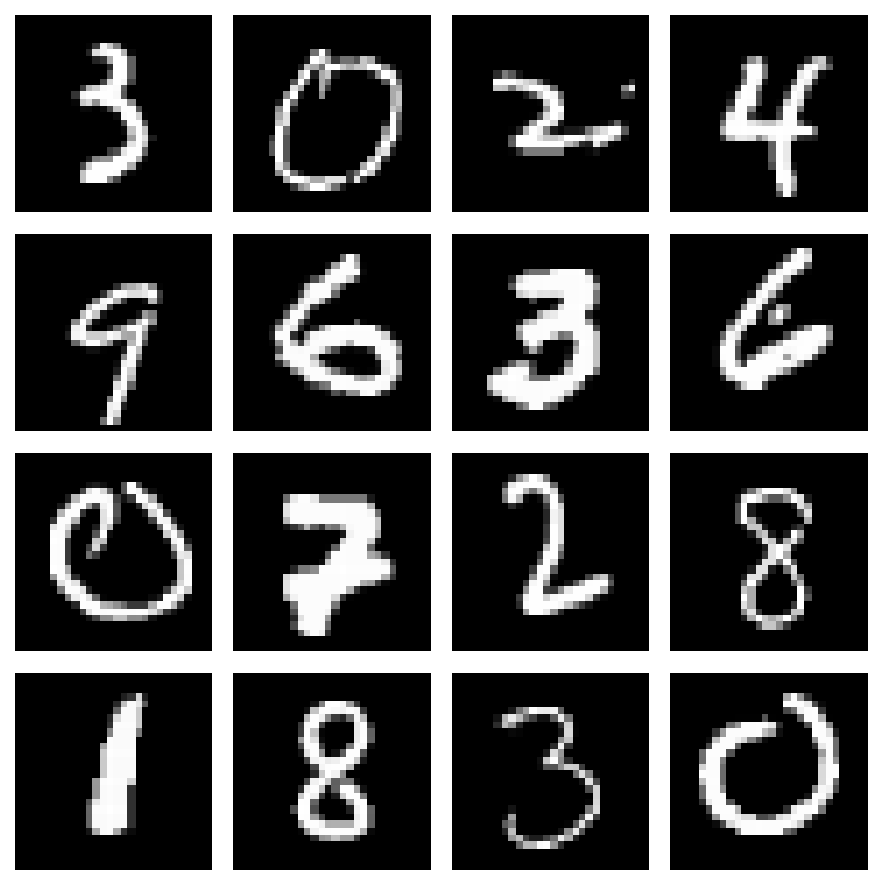
\includegraphics[width=.6\linewidth]{images/mnist.pdf}
      \caption{Random selection of images taken from the MNIST dataset \cite{bib:mnist}. The MNIST dataset consists of 28x28 grayscale images of handwritten digits from 0-9 and has 60000 training examples and 10000 testing examples.}
\label{fig:mnist}
\end{figure}
\FloatBarrier

\begin{figure}[!htb]
    \centering
  \begin{minipage}[b]{.48\linewidth}
      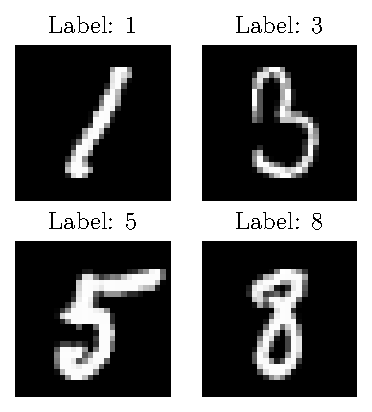
\includegraphics[width=\linewidth]{images/mnist_raw.pdf}
      \subcaption{Original.}
      \label{fig:mnist_dataset_original}
  \end{minipage}
  \begin{minipage}[b]{.48\linewidth}
      
\includegraphics[width=\linewidth]{images/mnist_binarized.pdf}
      \subcaption{Binarized.}
      \label{fig:mnist_dataset_binarized}
  \end{minipage}
  \caption{Part of sample from the original (\subref{fig:mnist_dataset_original}) and binarized (\subref{fig:mnist_dataset_binarized}) MNIST dataset. The original image is the number three and here we show a zoomed-in version(the upper right corner) to make the binarization visible. A LUT network can only do binary classification, so we have to binarize the labels as well. Numbers from 0-4 get the label 0 and numbers from 5-9 get the label 1.}
\label{fig:mnist_dataset}
\end{figure}
\FloatBarrier

\subsection{Experiments from paper}
We construct a LUT network with five hidden layers and 1024 LUTs per hidden layer. Every LUT in the network takes eight bits as input. Construction of the network is performed using the training set with 60000 samples and after training we validate on the test set with 10000 samples. The code is written by ourselves in Python using the package Numpy \cite{bib:harris2020array} for matrix operations. Similar to other machine learning packages, a LUT network object with provided arguments is first created and methods like \hl{\texttt{.train()}} and \hl{\texttt{.predict()}} allows the user to work with the LUT network at a high level. The code is available on GitHub \cite{bib:lut_github}. We obtain a training accuracy of 0.89 and a test accuracy of 0.87 which are the exact results from \cite{bib:chatterjee2018learning}. Note that the results are way above 0.5 meaning some learning had taken place. The way the LUT network is defined, every individual LUT already gives a prediction on the example passed to the network. That means we can compute the accuracy of every LUT in the network. Figure~\ref{fig:ex1_depth_performance} visualizes the training accuracy dependent on the layer. Each point represents the mean training accuracy over the respective layer and the total height of the error bars are two standard deviations. We can see that with increasing layer number, the accuracy goes up and the standard deviation goes down until it reaches zero at layer six because there is only one LUT in the last layer. Increasing performance with increasing depth reminds us of neural networks where adding more layers is a heuristic to increase performance.

\begin{figure}[!htb]
    \centering
    \includestandalone[]{standalone/lut/depth_performance}
    \caption{Training accuracy dependent on the layer for an 8-LUT network with five hidden layers (six is the output layer with just one LUT) and 1024 LUTs per hidden layer, trained on the Binary-MNIST dataset using our own code \cite{bib:lut_github}. The points represent the mean over the respective layer with two standard deviations as total height of the error bars. Similar to neural networks, we can see that performance increases with increasing depth. These results are our own and are almost identical to \cite{bib:chatterjee2018learning}.}
\label{fig:ex1_depth_performance}
\end{figure}
\FloatBarrier

\noindent The bit-size of the LUTs (denoted by $\delta$ in Algorithm~\ref{alg:LUT}) is a crucial hyperparameter. In another experiment, \cite{bib:chatterjee2018learning} varies the bit-size from two to 16 with steps of two and observes the effect on training and testing accuracy. The rest of the LUT network is the same as before. Figure~\ref{fig:ex1_k_acc} visualizes the results.

\begin{figure}[!htb]
    \centering
    \includestandalone[]{standalone/lut/k_acc_real}
    \caption{Training and testing accuracy on Binary-MNIST when the bit-size of a LUT newtwork with five hidden layers and 1024 LUT per hidden layer is varied. Increasing the bit-size sufficiently drives the training accuracy near perfection. As with machine learning models in general, the testing accuracy goes down with too much complexity, meaning we are overfitting. The underlying data to produce this plot is taken from \cite{bib:chatterjee2018learning}.}
\label{fig:ex1_k_acc}
\end{figure}
\FloatBarrier

\subsection{Varying the number of LUTs per hidden layer} \label{sec:num_luts_per_layer}
Throughout this thesis, we will stick with LUT networks with five hidden layers and 1024 LUTs per hidden layer to stay consistent with \cite{bib:chatterjee2018learning}. We will now invesigate what effect changing only the number of LUTs per hidden layer has. We use an 8-LUT network with five hidden layers and evaluate the accuracy at $2^i$ LUTs per layer, where $i = 1, \dots, 12$. The result can be seen in Figure~\ref{fig:num_luts_per_layer}, where Figure~\ref{fig:num_luts_per_layer:num} has an arithmetic scale and Figure~\ref{fig:num_luts_per_layer:num_log} has a logarithmic scale. We can see that going above 512 LUTs per hidden layer does not increase the accuracy anymore. In Section~\ref{sec:lut_network_size} we have seen that the number of LUTs per hidden layer is linearly proportional to the LUT network size on disk. So although not as important as the bit-size, which influences the LUT network size exponentially, reducing the number of LUTs per hidden layer seems like a quick and easy way to reduce LUT network size, especially if the performance does not drop.

\begin{figure}[!htb]
    \centering
  \begin{minipage}[b]{.45\linewidth}
    \resizebox {1\textwidth} {!} {
    \includestandalone[]{standalone/lut/nlpl_num}
    }
    \subcaption{Arithmetic scale.}
    \label{fig:num_luts_per_layer:num}
  \end{minipage}
  \begin{minipage}[b]{.45\linewidth}
    \resizebox {1\textwidth} {!} {
    \includestandalone[]{standalone/lut/nlpl_num_log}
    }
    \subcaption{Logarithmic scale.}
    \label{fig:num_luts_per_layer:num_log}
  \end{minipage}
  \caption{Accuracy of an 8-LUT network with five hidden layers dependent on the number of LUTs per hidden layer, where (\subref{fig:num_luts_per_layer:num}) provides an arithmetic scale and (\ref{fig:num_luts_per_layer:num_log}) provides a logarithmic scale. Increasing the number of LUTs per hidden layer above 512 has no effect on the accuracy.}
\label{fig:num_luts_per_layer}
\end{figure}
\FloatBarrier

\subsection{Summary}
We introduced the concept of LUTs, which are classifiers working entirely in binary, from \cite{bib:chatterjee2018learning} by walking through a small example. A single LUT cannot grasp complex information and is limited in bit-size due to computational constraints, thus we considered LUT networks that are made of many individual LUTs. Using a binarized version of the MNIST dataset, which we call Binary-MNIST, we recreate one experiment from \cite{bib:chatterjee2018learning}, where our results match the ones from the paper. We also made ourselves aware that the bit-size influences the LUT (and thus LUT-network) size exponentially and that the number of LUTs per hidden layer can sometimes be reduced, resulting in a smaller size and almost no performance drop.

\section{Improving LUT-based architectures}
The LUT networks considered so far were able to learn something, but in order to be viable for real-world ML use, we have to improve the accuracy. Therefore, we now take the idea of LUT networks further and change things to try to improve the accuracy, where we take three main approaches:

\begin{itemize}
  \item modifying existing LUT networks or the LUT network learning algorithm,
  \item enhancing the dataset using feature-engineering and
  \item combining many LUT networks of low bit-sizes (ensembling).
\end{itemize}We will see that we are indeed able to improve the accuracy, where we obtain the best results with an ensembling technique. With an appropriate architecture choice, we are also able to keep model size low.

\subsection{Majority vote} \label{sec:majority_vote}
So far the final prediction came from a single LUT that takes its inputs from the last hidden layer. Considering the same architecture as in the previous section, the last hidden layer has 1024 LUTs. If the number of bits per LUT is eight, then for the final prediction only eight of all 1024 LUTs will be used. Since every LUT is trained with the same label vector $\bm{y}$, each of the 1024 LUTs could theoretically be used for a final prediction too. That motivates us to try a \textit{wisdom of the crowd} technique, a majority vote mechanism that takes into account the predictions of all LUTs in the last hidden layer. The prediction that occurs most often will be chosen as the final one. The complete scheme can be seen in Algorithm~\ref{alg:majority_vote}. We conduct an experiment using a LUT network with five hidden layers and 1024 LUTs per hidden layer, varying the bit-size from two to 10 with steps of one, predicting with and without majority vote each time. The result can be seen in Figure~\ref{fig:majority_vote}. We can see that for a low bit-size, using a majority vote significantly boosts the training and testing accuracy. For high bit-sizes, a majority vote has less effect, but still enhances the testing performance a little. Interestingly, at five bits per LUT all accuracies coincide. Since using a majority vote requires almost no extra computational effort and at worst the results stay the same, it seems to be a good technique for enhancing the network's performance.

\begin{algorithm}
  \caption{LUT network majority vote}
  \label{alg:majority_vote}
  \begin{algorithmic}
    \State Given binary vector $\bm{x}$ and trained LUT network according to Algorithm~\ref{alg:LUT} with $l_L$ LUTs in the last hidden layer, perform a majority vote to predict.
    \vspace{1em}
    \State Initialize empty list $\alpha = [\hspace{0.3em}]$
    \For{$i=1, \dots, j_L$}
      \State Append prediction of LUT$_i$ on $\bm{x}$ to $\alpha$ (either 0 or 1)
    \EndFor
    \If{$\sum\limits_{\alpha_i = 0} > \sum\limits_{\alpha_i = 1}$}
      \State Return 0
    \ElsIf{$\sum\limits_{\alpha_i = 0} < \sum\limits_{\alpha_i = 1}$}
      \State Return 1
    \Else
      \State Return random choice of $\{0, 1\}$
    \EndIf
  \end{algorithmic}
\end{algorithm}
\FloatBarrier

\begin{figure}[!htb]
    \centering
    \includestandalone[]{standalone/lut/majority_vote}
    \caption{Training and testing accuracies with and without using a majority vote mechanism for a LUT network with five hidden layers and 1024 LUTs per hidden layer. The task is Binary-MNIST. For low bit-sizes, using a majority vote significantly enhances performance while the effect lessens with higher bit-sizes, but still enhances the testing accuracy a little. Interestingly, all accuracies coincide at five LUTs per hidden layer.}
\label{fig:majority_vote}
\end{figure}
\FloatBarrier

\subsection{Maximizing layer-wise mean accuracy while training} \label{sec:max_layer_acc}
As mentioned earlier, every LUT is trained with the same label vector $\bm{y}$ and is able to give a prediction. With increasing hidden layer, the LUTs get increasingly better. Figure~\ref{fig:acc_layer_normal} visualizes this using histograms. The underlying data is the training accuracy per LUT per hidden layer for an 8-LUT network with five hidden layers and 1024 LUTs per hidden layer applied on the Binary-MNIST dataset. The training accuracy of this LUT network is 0.89 and the testing accuracy is 0.87, the same accuracies as in the first experiment. The $x$-axis represents the training accuracy. For each hidden layer, we divide the data in 10 equally-sized bins (in terms of the accuracy) from the minimum to maximum value. Then for each bin, we erect a bar, where the height represents the number of data points that fall into this bin. We can see that on average, the accuracy increases with hidden layer number and the spread of accuracies reduces dramatically. For hidden layer 1, the accuracies are worst and the spread is maximal. The worst LUTs on hidden layer 1 are only slightly better than chance. That motivates us to conduct an experiment in which we try to maximize the accuracy of the LUTs while training.

We conceptualize following algorithm: after training a layer, we discard the $n$ worst LUTs in that layer and establish $n$ new LUTs that are hopefully better. We said \enquote{hopefully} because the learning algorithm takes a random subset of columns of the previous layer, leaving it to chance if a new LUT will perform better in terms of accuracy. After obtaining those $n$ new LUTs, we score every LUT and again discard the $n$ worst LUTs until the mean accuracy does not change anymore. We set a patience $p$, i.e., a number of iterations after no change in mean accuracy we will move onto the next layer. The implementation is described in Algorithm~\ref{alg:max_layer_acc}.

\begin{figure}[!htb]
    \centering
    \includestandalone[]{standalone/lut/acc_layer_normal}
    \caption{Histograms of training accuracies per hidden layer for an 8-LUT network with five hidden layers and 1024 LUTs per hidden layer. The task is Binary-MNIST. For each hidden layer, the data is divided into 10 equally sized bins from minimum to maximum value. For each range, we erect a bar with the height equal to the number of data points that fall within that range. The overall accuracy of this network is 0.89 on the training set and 0.87 on the testing set.}
\label{fig:acc_layer_normal}
\end{figure}
\FloatBarrier

\begin{algorithm}
  \caption{Maximizing layer-wise mean accuracy while training}
  \label{alg:max_layer_acc}
  \begin{algorithmic}
    \State Given binary features $\bm{X}$ with $N$ rows and binary label vector $\bm{y}$, construct a LUT network with $L$ hidden layers where the training accuracy in each hidden layer is maximized. This algorithm modifies Algorithm~\ref{alg:LUT}.
    \vspace{1em}
    \State Choose additional hyperparameters:
    \Statein Number of LUTs $n$ to discard after each iteration
    \Statein Patience $p \in \mathds{N}$
    \For{$i = 1, \dots, L$}
      \State Train layer $L$ as in Algorithm~\ref{alg:LUT}
      \State $\text{no\_change} \in \mathds{N} \gets 0$
      \State $\text{best} \in \mathds{R} \gets 0$
      \While{$\text{no\_change} < p$}
      \State Discard $n$ worst performing LUTs on $(\bm{X}, \bm{y})$
      \State Append $n$ new LUTs trained on $(\bm{X}, \bm{y})$ to the current layer
        \State $\text{accs} \in \mathds{R}^N \gets $ accuracy of each LUT on $(\bm{X}, \bm{y})$
        \State $\text{curr} \in \mathds{R} \gets \text{mean}(\text{accs})$
        \If{$\text{curr} > \text{best}$}
          \State $\text{best} \gets \text{curr}$
          \State $\text{no\_change} \gets 0$
          \Else
            \State $\text{no\_change} \mathrel{+}= 1$
        \EndIf
      \EndWhile
    \EndFor
    \State The single LUT after the last hidden layer is created as usual
  \end{algorithmic}
\end{algorithm}
\FloatBarrier

\noindent Starting another experiment, we again use an 8-LUT network with five hidden layers and 1024 LUTs per hidden layer and the Binary-MNIST dataset. We set $p=10$ and $n=50$. After running Algorithm~\ref{alg:max_layer_acc}, we obtain a training accuracy of 0.90 and a testing accuracy of 0.88, slightly better than before. In Figure~\ref{fig:acc_layer_discard} we can see the accuracies per hidden layer visualized using a histogram. Contrary to Figure~\ref{fig:acc_layer_normal}, the distributions are much more narrow now. After training we also tried prediction with a majority vote, but the accuracies did not change.

\begin{figure}[!htb]
    \centering
    \includestandalone[]{standalone/lut/acc_layer_discard}
    \caption{Histograms of training accuracies per hidden layer for an 8-LUT network with five hidden layers and 1024 LUTs per hidden layer, applied on Binary-MNIST. For this network, we applied Algorithm~\ref{alg:max_layer_acc} to try to improve performance, yielding an overall accuracy of 0.90 on the training set and 0.88 on the testing set. The results of this network are slightly better (increase of 1\% training and testing accuracy) compared to the same network without optimization. Contrary to Figure~\ref{fig:acc_layer_normal}, the distributions are much narrower.}
\label{fig:acc_layer_discard}
\end{figure}
\FloatBarrier

\noindent For a more complete picture, we vary the bit-size from two to 10 while applying Algorithm~\ref{alg:max_layer_acc}. There are again five hidden layers with 1024 LUTs per hidden layer. The result can be seen in Figure~\ref{fig:increase_layer_acc}. We can see that pushing up the layer-wise accuracy does indeed help increase the overall accuracy, albeit only significantly for low bit-sizes. For high bit-sizes, the effect is diminished.


\begin{figure}[!htb]
    \centering
    \includestandalone[]{standalone/lut/increase_layer_acc}
    \caption{Training and testing accuracies for LUT networks of varying bit-size with five layers and 1024 LUTs per hidden layer applied on Binary-MNIST. Solid lines and markers denote accuracies of networks where we applied Algorithm~\ref{alg:max_layer_acc}. For low bit-sizes, improving the layer-wise accuracies has a significant effect on the overall performance, while for higher bit-sizes the effect is diminished.}
\label{fig:increase_layer_acc}
\end{figure}
\FloatBarrier

\subsection{Feature engineering} \label{sec:feature_engineering}
So far we have not done any more sophisticated feature engineering except making a binary version out of the original MNIST dataset. Since feature engineering is an integral part of machine learning in general, we try it too and see if there is an improvement of the model's performance. We enhance the data by emphasizing the edges. Concretely, we create a copy of the original image and replace each pixel with black if the adjacent pixel has the same value and white if the adjacent pixel has a different value. We do this process both in $x$- and $y$-direction and add the results to the original image. Figure~\ref{fig:sobel_single} illustrates this technique for one example.

\begin{figure}[!htb]
    \centering
    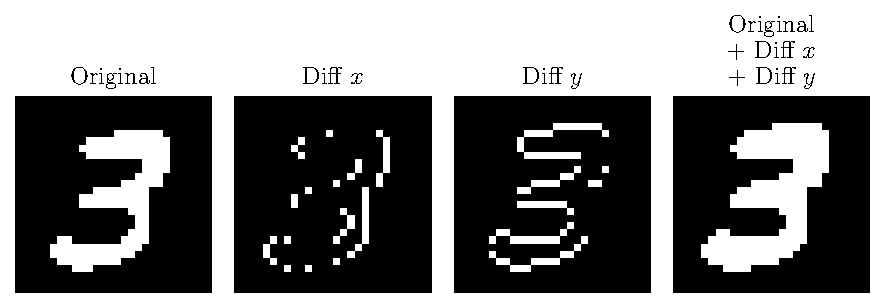
\includegraphics[width=.9\linewidth]{images/diff.pdf}
    \caption{Single example from the training data where we applied feature engineering. We create a copy of the original image and replace each pixel with black if the adjacent pixel has the same value and white if the adjacent pixel has a different value. We perform this process both in $x$- and $y$-direction and add the results to the original image. Looking at the feature-engineered image on the right, the number appears thicker.}
\label{fig:sobel_single}
\end{figure}
\FloatBarrier

\noindent Using the dataset enhanced with feature engineering, we train a LUT network with five hidden layers and 1024 LUTs per hidden layer, varying the bit-size from two to 10. The result can be seen in Figure~\ref{fig:sobel_acc}. We can see that the accuracies are consistently higher for models that were trained on images where feature engineering had been applied. The technique described in this section was inspired by the Sobel operator \cite{bib:sobelsobel} which calculates the gradients in an image in either $x$- or $y$-direction. Using this operator as feature engineering technique as opposed to our own produces similar results. We presented our own as main technique for the sake of an easier explanation and brevity.

\begin{figure}[!htb]
    \centering
    \includestandalone[]{standalone/lut/feature_engineering}
    \caption{Train and test accuracies for models trained on unmodified Binary-MNIST data and Binary-MNIST data where feature engineering had been applied. We can see that using feature engineering boosts the performance slightly.}
\label{fig:sobel_acc}
\end{figure}
\FloatBarrier


\subsection{Plain LUT ensembling} \label{sec:plain_lut_ensemble}
In Section~\ref{sec:majority_vote}, as opposed to having one final LUT, we counted the number of output labels in the last hidden layer and took that label as final prediction whichever was occurring the most. We could view that as a \textit{wisdom of the crowd} technique. Another approach is to bunch together $n$ separate LUT networks that do not use a majority vote and combine their prediction into one. We simply use that label as final prediction which was predicted the most out of the $n$ LUT networks. In the event that both labels occur the same number of times, we make a random choice. The scheme is described in detail in Algorithm~\ref{alg:lut_ensemble}.

We conduct an ensembling experiment where we use 2-LUTs as base classifiers. Keeping the bit-size low allows us to increase the number of individual LUT networks to a much higher degree. Training and inference for 8-LUT networks would take too long, at least with our current code. Figure~\ref{fig:plain_lut_ensembling} visualizes the result of the experiment. We use LUT network ensembles with $2^{1, \dots, 10}$ individual LUT classifiers. At just two LUT networks, the training accuracy is fairly low at 0.68, as it would be with a single 2-LUT network. Increasing the number of LUT networks increases the training accuracy and a peak at 0.78 with 64 LUTs is reached. Increasing the number of LUTs even more has no effect on the accuracy. Interestingly, the testing accuracy is consistently higher than the training accuracy.

\begin{algorithm}
  \caption{LUT ensembling}
  \label{alg:lut_ensemble}
  \begin{algorithmic}
    \State Given trained $\text{LUT}_{1, \dots, n}$, perform ensembling to predict on yet unseen $\bm{x}$.
    \vspace{1em}
    \State Initialize empty list $\alpha = [\hspace{0.3em}]$
    \For{$i=1, \dots, n$}
      \State Append prediction of LUT$_i$ on $\bm{x}$ to $\alpha$ (either 0 or 1)
    \EndFor
    \If{$\sum\limits_{\alpha_i = 0} > \sum\limits_{\alpha_i = 1}$}
      \State Return 0
    \ElsIf{$\sum\limits_{\alpha_i = 0} < \sum\limits_{\alpha_i = 1}$}
      \State Return 1
    \Else
      \State Return random choice of $\{0, 1\}$
    \EndIf
  \end{algorithmic}
\end{algorithm}
\FloatBarrier

\begin{figure}[!htb]
    \centering
    \includestandalone[]{standalone/lut/plain_lut_ensembling}
    \caption{Train and test accuracies for LUT network ensembles according to Algorithm~\ref{alg:lut_ensemble} on Binary-MNIST. The base classifiers are 2-LUT networks with five hidden layers and 1024 LUTs per hidden layer. Training and testing accuracies reach a peak at 64 LUT networks, increasing the LUT number even more has no effect on the accuracy. Interestingly, the testing accuracy is consistently higher than the training accuracy.}
\label{fig:plain_lut_ensembling}
\end{figure}
\FloatBarrier

\subsection{Advanced LUT ensembling} \label{sec:ada_boost}
Now we try another ensembling method which is very well established in literature and practice, the AdaBoost.M1 algorithm \cite{bib:adaboostm1} which can be seen in Algorithm~\ref{alg:adaboostm1}. As the scheme in the previous Section~\ref{sec:plain_lut_ensemble}, AdaBoost.M1 combines predictions of $n$ separate classifiers $f_{1, \dots, n}$ into one. Every classifier is trained individually with the addition of weights $\bm{w}$, where $w_k > 0$. Every sample $k$ in the training set is assigned weight $w_k = 1/N$ in the beginning, where $N$ is the number of samples. The weights represent how much attention during training a single example should get, the higher the weight, the more attention the sample gets. Since all weights are equal in the beginning, every sample gets the same amount of attention in the first iteration. Once iteration $i$ is finished, a number $\alpha_i \in \mathds{R}$ is computed. If $\alpha_i > 0$, then the classifier is better than random and if $\alpha_i < 0$, then the classifier is worse than random. Using $\alpha_i$, we update each weight of only those samples which were misclassified. If the classifier is better than random, then we can do some fine-tuning and focus more on the misclassifications which corresponds to assigning higher weights to misclassified samples. If the classifier is worse than random, then we are not yet ready for fine-tuning and we should focus more on the most important samples which corresponds to assigning lower weights to misclassified samples. After $n$ iterations, training is finished and we can predict on yet unseen sample $\bm{x}$ using $\text{sign}(\sum_{i=1}^n \alpha_i f_i(\bm{x}))$. 

\begin{algorithm}
  \caption{AdaBoost.M1 algorithm according to \cite{bib:adaboostm1}} \label{alg:adaboostm1}
  \begin{algorithmic}[1]
    \State Given dataset $(\bm{X}, \bm{y})$, where $\bm{X} = \bm{x}_1, \dots, \bm{x}_N$ and $\bm{y} = y_1, \dots, y_N$, $y_i \in \{-1, 1\}$ and model class, construct a classifier that is made up of $n$ individual classifiers $f_1, \dots, f_n$.
    \vspace{1em}
    \State Initialize weight vector $\bm{w} \in \mathds{R}^N$ with $w_{1, \dots, N} = 1/N$
    \vspace{0.5em}
    \For{$i = 1, \dots, n$}
    \State Train classifier $f_i$ on $(\bm{X},\bm{y})$ and weights $\bm{w}$ \label{alg_line:adaboostm1:train}
    \State $\text{err}_i \gets \big( \sum_{k=1}^N w_k \mathbb{1}(f_i(\bm{x}_k) \neq y_k) \big) / \sum_{k=1}^N w_k$
    \State $\alpha_i = \log((1 - \text{err}_i) / \text{err}_i)$
    \For{$k = 1, \dots, N$}
    \State $w_k \gets w_k \exp(\alpha_i \mathbb{1}(f_i(\bm{x}_k) \neq y_k))$
    \EndFor
    \EndFor
    \State Prediction on yet unseen $\bm{x}$: $\text{sign} \big( \sum_{i = 1}^n \alpha_i f_i(\bm{x}) \big)$
  \end{algorithmic}
\end{algorithm}
\FloatBarrier

\noindent Using AdaBoost.M1 with LUT networks only works if we modify the algorithm slightly. Looking at Algorithm~\ref{alg:adaboostm1} on line~\ref{alg_line:adaboostm1:train}, we notice that there is no way to incorporate weights into the LUT learning algorithm (see Algorithm~\ref{alg:LUT}). Therefore, instead of training on all samples $\bm{X}$ with weights at each iteration, we train on a subset of samples $\bm{X}' \subset \bm{X}$ with fixed size $\rho \in \{1, \dots, N\}$ without weights. By choosing those samples with highest weights to be included in $\bm{X}'$, we are able to give more attention to those samples. The modified AdaBoost.M1 for LUT networks can be seen in Algorithm~\ref{alg:lut_ensemble_ada}. The modifications take place from line~\ref{alg_ref:lut_ensemble_ada:mod_begin} to line~\ref{alg_ref:lut_ensemble_ada:mod_end}. On the first iteration, we train on the entire dataset. On all other iterations, we train on $\rho$ samples with the highest weights. The command $\text{argsort}(\bm{w})$ returns indices that would sort $\bm{w}$. We are interested in the highest weights, not the lowest ones, so we reverse the sorted indices: $\text{reversed}(\text{argsort}(\bm{w}))$. We then take a subset, the first $\rho$ entries: $\text{reversed}(\text{argsort}(\bm{w}))[:\rho]$. Now we have the indices of $\rho$ samples with highest weights and take a subset of the dataset: $\bm{X}[\text{idxs}]$ and $\bm{y}[\text{idxs}]$.

\begin{algorithm}
  \caption{LUT ensembling inspired by AdaBoost.M1}\label{alg:lut_ensemble_ada}
  \begin{algorithmic}[1]
    \State Given dataset $(\bm{X}, \bm{y})$, where $\bm{X} = \bm{x}_1, \dots, \bm{x}_N$ and $\bm{y} = y_1, \dots, y_N$, $y_i \in \{-1, 1\}$, construct a classifier that is made up of $n$ individual classifiers $\text{LUT}_{1, \dots, n}$.
    \vspace{1em}
    \State Initialize weight vector $\bm{w} \in \mathds{R}^N$ with $w_{1, \dots, N} = 1/N$
    \State Choose $\rho$ out of $\{1, \dots, N\}$
    \vspace{0.5em}
    \For{$i = 1, \dots, n$} \label{alg_ref:lut_ensemble_ada:mod_begin}
    \If{i = 1}
      \State Train $\text{LUT}_i$ on $(\bm{X},\bm{y})$
    \Else
    \State $\text{idxs} = \text{reversed}(\text{argsort}(\bm{w}))[:\rho]$
    \State $\bm{X}' \subset \bm{X} \gets \bm{X}[\text{idxs}]$
    \State $\bm{y}' \subset \bm{y} \gets \bm{y}[\text{idxs}]$
      \State Train $\text{LUT}_i$ on $(\bm{X}', \bm{y}')$
      \EndIf \label{alg_ref:lut_ensemble_ada:mod_end}
    \State $\text{err}_i \gets \big( \sum_{k=1}^N w_k \mathbb{1}(\text{LUT}_i(\bm{x}_k) \neq y_k) \big) / \sum_{k=1}^N w_k$
    \State $\alpha_i = \log((1 - \text{err}_i) / \text{err}_i)$
    \For{$k = 1, \dots, N$}
    \State $w_k \gets w_k \exp(\alpha_i \mathbb{1}(\text{LUT}_i(\bm{x}_k) \neq y_k))$
    \EndFor
    \EndFor
    \State Prediction on yet unseen $\bm{x}$: $\text{sign} \big( \sum_{i = 1}^n \alpha_i \text{LUT}_i(\bm{x}) \big)$
  \end{algorithmic}
\end{algorithm}
\FloatBarrier

\noindent We apply Algorithm~\ref{alg:lut_ensemble_ada} and use 2-LUT networks with five hidden layers and 1024 LUTs per hidden layer and choose $\rho = N/5$. We vary the number of LUT networks from 2 to 1024. The motivation for choosing 2-LUT networks is computation time and disk size. Since we want to keep open the possibility for many LUT networks in the ensembled classifier, we have to restrict ourselves with the bit-size, otherwise it would take too long to train and predict. Our overall goal also includes a small disk size. A LUT network ensemble of 8-LUTs with five hidden layers and 1024 LUTS per hidden layer would take up 168 MB of space, way out of proportions. The results can be seen in Figure~\ref{fig:ada_2_LUT}. We can see that with an increasing number of LUT networks, we can indeed improve the accuracy. At 1024 LUT networks, we achieve a training accuracy of 0.94 and testing accuracy of 0.93. When it comes to the testing accuracy, this is the best result so far. Interesting is the lack of a significant difference between training and testing accuracies. Usually there is a point where overfitting starts to take place and the testing accuracy decreases compared to the training accuracy. Perhaps overfitting will take place at more LUT networks than 1024, but we do not go above that because it would take too much time to train for us. However, a LUT network ensemble of 2-LUTs with five hidden layers and 1024 LUTs per hidden layer takes up 2.62 MB of disk space, larger than the CNN we used before which was 1.16 MB in size. We therefore evaluate training and testing performance on a 2-LUT ensemble with five hidden layers and only 64 LUTs per hidden layer. This architecture takes up only 168 KB of disk space. We obtain a trainig and testing accuracy of 0.94.

\begin{figure}[!htb]
    \centering
    \includestandalone[]{standalone/lut/ada_2_LUT}
    \caption{Training and testing accuracies for ensembles of 2-LUT networks with five hidden layers and 1024 LUTs per hidden layer according to Algorithm~\ref{alg:lut_ensemble_ada}. At 1024 LUT networks, we obtain training and testing accuracies of 0.94 and 0.93, respectively, best so far when it comes to testing accuracy. Notice the lack of significant difference between training and testing accuracy as it would be when overfitting. Perhaps overfitting takes place at more individual LUTs. Using 1024 LUT networks per hidden layer make the size of this ensemble be 2.62 MB which is bigger than the CNN with 1.16 MB we used before. Performing another experiment with an ensemble of 1024 2-LUT networks with five hidden layers and only 64 LUTs per hidden layer, we obtain a training and testing accuracy of 0.94 and this architecture only takes up 168 KB of space.}
\label{fig:ada_2_LUT}
\end{figure}
\FloatBarrier

\noindent As opposed to LUT architectures in previous sections, the AdaBoost.M1 inspired ensemble requires floating-point computations to make predictions ($\alpha_i$ in Algorithm~\ref{alg:lut_ensemble_ada}). LUTs and LUT networks can be implemented fast on a binary level, since for inference, we just have to look up entries in tables. The floating-point computation here further complexifies inference, however, we will not investigate to what degree speed is influenced.

\subsection{Combining different methods}
We combine different methods presented in previous sections to try to push the accuracies even further. We utilize an AdaBoost.M1 inspired LUT classifier from Section~\ref{sec:ada_boost} with 1024 individual 2-LUT networks that each have 5 hidden layers and 64 LUTs per hidden layer. Additionally, we apply Algorithm~\ref{alg:max_layer_acc} to each LUT network while training and also use the feature-engineered dataset from Section~\ref{sec:feature_engineering}. For the hyperparameters, we set $\rho = N/5$, the number of LUTs to discard after each iteration $n=10$ and patience $p=10$. We obtain a training accuracy of 0.75 and testing accuracy of 0.78, worse than the results from Section~\ref{sec:ada_boost}. The results make us question Algorithm~\ref{alg:max_layer_acc}. It is interesting though that pushing up the accuracies of individual LUTs in LUT networks leads to an overall inferior performance when constructing an ensembled classifier.

\subsection{Summary}
Starting with a LUT-network architecture from \cite{bib:chatterjee2018learning}, we tried to make improvements in terms of accuracy and size which were successful. A majority vote and maximizing the layer-wise mean accuracy while training help improving performance of single LUT networks of low bit-size, for higher bit-sizes, however, the change does not surpass 1-2\%. Feature engineering gave small improvements in accuracy. Ensembling techniques are promising, especially an AdaBoost.M1 ensemble achieved a testing accuracy of 0.94, better than any previous single LUT networks. With a good choice of architecture, we were able to reduce the size of the ensemble significantly while retaining accuracy. However, the advance ensembling scheme requires floating-point computations again, albeit few. We also obtained results that suggest combining ensembling and maximizing the layer-wise mean accuracy is not a good idea. What we have not discussed is pruning of LUT networks, i.e. discarding individual LUTs that do not contribute to the final prediction. We have also not discussed multi-class classification which would be possible with LUTs using an one-vs-one or one-vs-all approach similar to SVMs \cite{bib:bishop2006pattern}.

\section{And-inverter graphs (AIGs)}
We will now consider another scheme of building a circuit. First we will introduce the concept of an AIG and how it can be used to predict something. Then, we will devise an initialization scheme and heuristic local search algorithm that we try out by running experiments. We will find that the local search algorithm works and we are able to iteratively improve the accuracy. The resulting AIGs are very small (way below 1 Kilobyte), so their implementation on devices with little computing power is promising. What remains to be done is to try out better search algorithms that find AIGs with higher accuracies and are faster.

\subsection{Introduction}
Let us start by introducing another predictive system that looks like a network and works with binary values. Consider binary variable $\mathsf{2}$. For consistency, which will become apparent later on, we will use numeric variables. It can either be true or false. Introducing another variable $\mathsf{4}$, we can perform a logical operation on $\mathsf{2}$ and $\mathsf{4}$, similar to how we can perform a mathematical operation with two real numbers (e.g., adding, subtracting, dividing them, etc.). Logical operators include AND ($\wedge$), OR ($\vee$), IMPLICATION ($\Rightarrow$), XOR ($\otimes$) and so on. If we compute

\begin{align} \label{eq:ceqaandb}
    \mathsf{12} = \mathsf{2} \wedge \mathsf{4},
  \end{align}where $\mathsf{12}$ is another binary variable, we can visualize this using a graph, visible in Figure~\ref{fig:aig1}. First let us consider Figure~\ref{fig:aig1-text}. We interpret variables $\mathsf{2}$ and $\mathsf{4}$ as \textit{inputs} and thus draw them using boxes and label them additionally using triangle nodes. Variable $\mathsf{6}$ in Equation~\ref{eq:ceqaandb} becomes and \textit{and-node}, i.e., it is the result of performing AND on $\mathsf{2}$ and $\mathsf{4}$, and we denote it using a circular node. Since variable $\mathsf{12}$ is already the output of equation~\ref{eq:ceqaandb}, we mark it using a triangle node. We could already imagine Equation~\ref{eq:ceqaandb} being a predictive system. Suppose we want to build a predictive system that forecasts whether or not teenage boy \enquote{Hans} will refresh himself at the family's swimming pool. We are his neighbors and have good information about his daily life, albeit limited. We observe that on a hot and sunny day, he is almost always at the pool. Thus we assign $\mathsf{2}$ to true if it is sunny and false otherwise and $\mathsf{4}$ to true if it is hot and false otherwise. Variable $\mathsf{12}$ now represents our prediction if Hans will go to the pool. Figure~\ref{fig:aig1-text} visualizes this predictive system.

\begin{figure}[!htb]
    \centering
  \begin{minipage}[b]{.3\linewidth}
    \centering
    \resizebox {0.63\textwidth} {!} {
      \includestandalone[]{standalone/aig/aig1-num}
    }
    \subcaption{Plain tree.}
    \label{fig:aig1-num}
  \end{minipage}
  \begin{minipage}[b]{.5\linewidth}
    \centering
    \resizebox {0.5\textwidth} {!} {
      \includestandalone[]{standalone/aig/aig1-text}
    }
    \subcaption{Tree with interpretation of variables.}
    \label{fig:aig1-text}
  \end{minipage}
\caption{Equation~\ref{eq:ceqaandb} visualized using a graph in (\subref{fig:aig1-num}) with a possible meaning to the variables in (\subref{fig:aig1-text}). Inputs are drawn using a box node and further labeled using triangle nodes. Circular nodes perform AND on two other nodes which can be either input nodes or other AND nodes. Outputs are denoted using triangle nodes. In (\subref{fig:aig1-num}), the same object is represented, but this time a meaning to the variables is given. We predict teenage boy Hans to go to the pool if it is sunny and hot.}
\label{fig:aig1}
\end{figure}
\FloatBarrier

\noindent Looking at Figure~\ref{fig:aig1-text}, we notice that it looks like an upside-down tree that has two branches. Consequently, given any node, nodes that are connected and above it we call \enquote{parents}. For example, variable $\mathsf{12}$ is the parent of variable $\mathsf{2}$ and $\mathsf{4}$ because it is further down in the tree. Nodes that are below a node and connected to it we call \enquote{children}, so variables $\mathsf{2}$ and $\mathsf{4}$ are children of variable $\mathsf{12}$.

\noindent We will now consider more complexity in our predictive system. We observe that on some days, Hans is mowing the lawn instead of relaxing at the pool, surely because his parents told him to do so. If binary variable $\mathsf{6}$ represents whether or not Hans has to mow the lawn, we can update our predictive system:

\begin{align} \label{eq:aig2}
  \mathsf{16} = \lnot \mathsf{6} \wedge (2 \wedge 4).
\end{align}, where the symbol $\lnot$ denotes negation and variable $\mathsf{16}$ is the new output. The visualization of Equation~\ref{eq:aig2} using a graph can be seen in Figure~\ref{fig:aig2}. There is a new input (I2) with a black dot at the connection to the next node. This black dot denotes negation.

\begin{figure}[!htb]
    \centering
  \begin{minipage}[b]{.3\linewidth}
    \centering
    \resizebox {0.875\textwidth} {!} {
      \includestandalone[]{standalone/aig/aig2-num}
    }
    \subcaption{Plain tree.}
    \label{fig:aig2-num}
  \end{minipage}
  \begin{minipage}[b]{.6\linewidth}
    \centering
    \resizebox {0.8\textwidth} {!} {
      \includestandalone[]{standalone/aig/aig2-text}
    }
    \subcaption{Tree with interpretation of variables.}
    \label{fig:aig2-text}
  \end{minipage}
\caption{Predictive system from Figure~\ref{fig:aig1} with complexity added. There is now another binary variable \enquote{Have to mow the lawn} which is an input. The black dot denotes negation. What was previously the output of the system becomes an intermediate result: \enquote{Want to go to the pool}.}
\label{fig:aig2}
\end{figure}
\FloatBarrier

\noindent Lets us now consider even more complexity. We know that Hans has a sister and sometimes we would find her alone at the pool on a hot and sunny day, but we never observe the two being together there. On one occasion, we see that Hans chases her away from the pool with his Friend. Hans' friend is not over as much as he could be and we have in vague memory that he is an avid baseball fan. We thus come up with folliwing reasoning: Hans does not like being at the pool with his sister together, probably because he thinks she is annoying. But if his friend is over, he has the courage to chase her away. If a baseball game is on TV, Hans' friend will prefer to stay at home and watch it. The resulting predictive system is visualized in Figure~\ref{fig:aig3-num} with numeric variable names and in Figure~\ref{fig:aig3} with an interpretation given to the variables. We invite the reader to take some time studying it. The upper most part can be understood easily by considering that for boolean variables $A$ and $B$: $A \vee B \Leftrightarrow \lnot (\lnot A \wedge \lnot B)$.

\begin{figure}[!htb]
    \centering
    \resizebox {0.35\textwidth} {!} {
      \includestandalone[]{standalone/aig/aig3-num}
    }
    \caption{Predictive system if teenage boy Hans will go relax himself at the family's swimming pool, with more complexity added.}
\label{fig:aig3-num}
\end{figure}
\FloatBarrier

\begin{figure}[!htb]
    \centering
    \resizebox {0.65\textwidth} {!} {
      \includestandalone[]{standalone/aig/aig3-text}
    }
    \caption{Predictive system if teenage boy Hans will go relax himself at the family's swimming pool, with more complexity added. Here we wrote an interpretation to each node. The upper most part can be understood easily by considering that for boolean variables $A$ and $B$: $A \vee B \Leftrightarrow \lnot (\lnot A \wedge \lnot B)$.}
\label{fig:aig3}
\end{figure}
\FloatBarrier

An interpretation, such as in Figure~\ref{fig:aig3} is usually not available to us. For example, in the case of the Binary-MNIST dataset, there are 784 possible inputs and a heuristic random search algorithm (that we will later introduce) searches for an AIG structure. Even if the meaning of each input is apparent to us, how these inputs are processed further down in the tree is hard to interpret. In the following sections, we will thus not try to come up with an interpretation of the trees.

Looking at Figure~\ref{fig:aig3}, it looks like we are dealing with facts and implication, but really this is a \textit{predictive system}, so its output is not guaranteed to be true. After all, we constructed this system with our own limited information. There are many more factors to consider if Hans will go to the swimming pool, such as homework, the pool being under maintemance, Hans prefering to play computer games indoor and so on. As with LUTs, a predictive system like this cannot handle uncertainty, i.e., what is the \textit{probability} of Hans going to the pool. The output is either 0 or 1. One solution would be to discretize the probability range, e.g., 0-25\%, 26-50\%, 51-75\%, 76-100\% and have a 2-bit output. In this thesis, however, we do not consider probabilistic output.

This new type of predictive systems introduced in this section are called \enquote{and-inverter graphs} (AIGs) \cite{bib:aig_wiki}. AIGs are used to represent logic functions and they can be easily implemented as circuits. We will use them in a machine learning context, i.e., given a training set with features and labels we search for an architecture that has the highest possible accuracy.

\subsection{Initialization of a random AIG}
First we must initialize a random AIG that we can later pass to the heuristic local search algorithm. We need a systematic way to build an AIG structure, where cyclicity is forbidden. We use an approach inspired from neural networks. A NN has a certain number of hidden layers and each hidden layer takes input only from the previous one. Thus there is never cyclicity. We take a similar approach for AIGs by specifying the number of hidden layers, the number of nodes per hidden layer and how many outputs there are. Each node takes two inputs (i.e., children $c_1$ and $c_2$) randomly from the previous hidden layer and the inputs to the node are randomly negated or not. Important to note is that almost all architectures initialized this way have \enquote{inactive nodes}, i.e. they do not contribute to the final prediction. Inactive nodes are still part of the architecture, though, and may become active during the search process. An AIG with all inactive nodes removed, we call a \enquote{pruned AIG}. Figure~\ref{fig:aig-init} visualizes a randomly initialized AIGs, where the inactive nodes are dotted. Algorithm~\ref{alg:aig_init} described the initialization process more formally. 

\begin{figure}[!htb]
    \centering
    \resizebox {0.45\textwidth} {!} {
      \includestandalone[]{standalone/aig/aig-init}
    }
    \caption{Randomly initialized AIG with inactive nodes (dotted). Inactive nodes do not contribute to the prediction, but may become active during the search process. Input nodes I1 and I3 also do not contribute to the prediction.}
\label{fig:aig-init}
\end{figure}
\FloatBarrier

\begin{algorithm}
  \caption{Random AIG initialization}
  \label{alg:aig_init}
  \begin{algorithmic}
    \State Given number of inputs $I$, number of hidden layers $L$, number of nodes per hidden layer $l_1, \dots, l_L$ and number of outputs $O$, construct a random AIG.
    \vspace{1em}
    \For{hidden layer $i = 1, \dots, L$}
      \For{node $l_1, \dots, l_L$}
        \State Choose $c_1$ randomly from any nodes in the previous layer
        \State Negate $c_1$ with a 50\% chance
        \State Choose $c_2$ randomly from any nodes in the previous layer,  where $c_2 \neq c_1$
        \State Negate $c_2$ with a 50\% change
      \EndFor
    \EndFor
    \For{output node $i = 1, \dots, O$}
      \State Choose $c_1$ randomly from any nodes in the last hidden layer
      \State Negate $c_1$ with a 50\% chance
      \State Choose $c_2$ randomly from any nodes in the hast hidden layer,  where $c_2 \neq c_1$
      \State Negate $c_2$ with a 50\% change
    \EndFor
  \end{algorithmic}
\end{algorithm}
\FloatBarrier

\subsection{Greedy local search}
Given our dataset and randomly initialized AIG, we would like an architecture that has the highest possible performance in terms of accuracy, meaning we need a search algorithm. We choose a greedy local search \cite{bib:koller2009probabilistic} because it is fairly simple and easy to implement, thus a great way to start. The basic idea is to consider a set of successor architectures. Such a set arises when we consider each active node in the graph and change a small thing, i.e., change a child to another node or negating a child. We score each architecture and take the one that has the highest training accuracy, thus proceeding to the next iteration. If the training accuracy does not improve for a certain number of iterations, we finish. The greedy local search is described in Algorithm~
\ref{alg:aig_local_search}.

\begin{algorithm}
  \caption{AIG greedy local search}
  \label{alg:aig_local_search}
  \begin{algorithmic}
    \State Given binary dataset $(\boldsymbol{X}, \bm{y})$ and randomly initialized AIG with architecture $\sigma_0$, perform a greedy local search.
    \vspace{1em}
    \State Choose hyperparameters:
      \Statein Patience $p$
    \State $\text{no\_change} \in \mathds{N} \gets 0$
    \State $s \in \mathds{R} \gets 0$
    \State $\sigma \gets \sigma_0$
    \While{$\text{no\_change} < p$}
      \State $\Sigma = [\hspace{0.3em}]$
      \State $S = [\hspace{0.3em}]$
      \For{all active nodes in $\sigma$}
          \State $\sigma' \gets$ change $c_1$ to any node in the previous layer
          \State $\Sigma.\text{append}(\sigma')$, $S.\text{append}(\text{accuracy\_score}(\sigma', (\bm{X}, \bm{y})))$
          \State $\sigma' \gets$ change $c_2$ to any node in the previous layer
          \State $\Sigma.\text{append}(\sigma')$, $S.\text{append}(\text{accuracy\_score}(\sigma', (\bm{X}, \bm{y})))$
          \State $\sigma' \gets$ change polarity of $c_1$
          \State $\Sigma.\text{append}(\sigma')$, $S.\text{append}(\text{accuracy\_score}(\sigma', (\bm{X}, \bm{y})))$
          \State $\sigma' \gets$ change polarity of $c_2$
          \State $\Sigma.\text{append}(\sigma')$, $S.\text{append}(\text{accuracy\_score}(\sigma', (\bm{X}, \bm{y})))$
      \EndFor
      \State $s' \gets \text{max}(S)$
      \If{s' > s}
        \State $s \gets s'$
        \State $\text{no\_change} \gets 0$
        \State $\sigma \gets \Sigma[\text{argmax}(S)]$
      \Else
        \State $\text{no\_change} \mathrel{+}= 1$
      \EndIf
    \EndWhile
  \end{algorithmic}
\end{algorithm}
\FloatBarrier

\subsection{Experiments}
We again use the Binary-MNIST dataset. We use the AIG format and library \enquote{AIGER} \cite{bib:Biere-FMV-TR-07-1} to specify and run our AIGs. The network structure and local search algorithm we have written from scratch in C++. Along with random initialization and the local search, the code features functionality to export into AIGER format and to export visualizations. The code is available on GitHub \cite{bib:aig_github}. Utilizing initialization from Algorithm~\ref{alg:aig_init} and training from Algorithm~\ref{alg:aig_local_search}, we run 42 experiments. There are 784 inputs and we choose 3 hidden layers with 64 AND nodes per hidden layer, meaning any resulting AIG will maximally have 192 AND-gates. The very low number of AND-gates that we permit is due to computational constraints, otherwise it would take too long. The output layer has one AND node and takes inputs from the last hidden layer. In Figure~\ref{fig:aig_exp_result}, 10 out of the 42 runs are visualized. The mean final training and testing accuracies of all runs are 0.65 and 0.66, respectively. The maximum final training and testing accuracies of all runs are 0.74 and 0.74, respectively. A summary can be seen in Table~\ref{tab:aig_accuracies}. A higher initial training accuracy does not necessarily mean a higher final accuracy. A visualization of the pruned best AIG found can be seen in Appendix~\ref{app:aig-mnist}.

\begin{figure}[!htb]
    \centering
  \begin{minipage}[b]{.49\linewidth}
    \resizebox {1\textwidth} {!} {
    \includestandalone[]{standalone/aig/aig_exp_result_train}
    }
    \subcaption{Training.}
    \label{fig:aix_exp_result:train}
  \end{minipage}
  \begin{minipage}[b]{.49\linewidth}
    \resizebox {1\textwidth} {!} {
    \includestandalone[]{standalone/aig/aig_exp_result_test}
    }
    \subcaption{Testing.}
    \label{fig:aig_exp_result:test}
  \end{minipage}
  \caption{Results (training accuracies) of greedy local search according to Algorithm~\ref{alg:aig_local_search} on AIGs. We performed 38 experiments, 10 of which are visualized here. The initial training accuracies vary from 0.61 to 0.61. A higher initial training accuracy does not necessarily mean a higher final accuracy. Best of all runs was 0.77.}
\label{fig:aig_exp_result}
\end{figure}
\FloatBarrier

\begin{table}[!htb]
  \centering
\begin{tabular}{lll}
                      & Train & Test \\ \hline
Mean initial accuracy & 0.54  & 0.55 \\
Min initial accuracy  & 0.51  & 0.51 \\
Max initial accuracy  & 0.64  & 0.66 \\
Mean final accuracy   & 0.65  & 0.66 \\
Min final accuracy    & 0.51  & 0.51 \\
Max final accuracy    & 0.74  & 0.74
\end{tabular}
\caption{Statistics over initial and final training and test accuracies out of the 42 runs in which we performed an AIG local serach.}
\label{tab:aig_accuracies}
\end{table}

\begin{figure}[!htb]
  \centering
  \resizebox {.8\textwidth} {!} {
    \includestandalone[]{standalone/aig/best_aig_pruned}
  }
  \caption{Best AIG found using a greedy local search. Due to a bug in our code, node 1734 takes two identical inputs which is normally not permitted. Nevertheless, it has a testing accuracy of 0.745, just a little over the second best AIG with a testing accuracy of 0.742. It is interesting that an AIG this small still generalizes, albeit with low accuracy.}
  \label{fig:best_aig}
\end{figure}
\FloatBarrier

\noindent We can see that we are able to improve the accuracy iteratively. With AIGs, the greedy local search algorithm is probably too optimistic, though, since we quickly bump into an upper ceiling. What also happens is to get stuck at sub-optimal areas, from which the accuracy never recovers. For example, in Figure~\ref{fig:aig_exp_result}, we can see a run that starts at a very low accuracy and never goes up at all. So there is need for a different search algorithm.

The extremely small size of the AIGs is promising. With the architecture chosen for the experiment, a single AIG only has 68 Bytes of disk size (we arrived at this number by converting an ASCII-encoded AIG file to binary using AIGER and looking at the file size). A small size, together with the lack of need for floating-point matrix computations, make these architectures extremely fast and thus suitable for electronic devices with very little computing power. Furthermore, AIGs are easily translatable to circuits that are implemented on hardware, so the architecture could be much bigger.

\subsection{Summary}
We introduced AIGs and investigated whether or not they can be used as predictive systems, where we have found that this is possible. We conceptualized our own initialization scheme and chose a greedy local search as search algorithm. We wrote the code for our experiments in C++ from scratch, making use of the AIGER library. Choosing an architecture that has maximally just 192 AND-gates, the best local search run returned an AIG that has an accuracy of 0.76 which is significantly above chance, meaning learning had taken place. The extremely small size, together with the prospect of implementation on hardware make AIGs very promising. Future work should consist of trying to find better search algorithms that are able to find better architectures in less time.

\section{Comparison of models}
To get an overview in terms of LUT-based models, AIGs and other common ML algorithms, we evaluate training and testing accuracies and model size, i.e. we create the data from which Figure~\ref{fig:model_performance} is generated. The convolutional neural network has the highest accuracy, but is bigger and requires floating-point matrix operations. Given the right choice of architecture and algorithm, LUT-based models are performing quite well, considering reduced size and possible bit-level implementation. The best AIG that we found lacks good accuracy compared to most other models, but is nevertheless very promising with its ultra-small file size of just 68 Bytes.

\subsection{Accuracy and size} \label{sec:models}
As in \cite{bib:chatterjee2018learning}, we train various machine learning algorithms on the Binary-MNIST dataset and compare their performance. The training and testing accuracies can be seen in Table~\ref{tab:ml_algos_on_bmnist} and testing accuracies are visualized in Figure~\ref{fig:model_performance}. Each LUT network has five hidden layers and 1024 LUTs per hidden layer, except the \enquote{8-LUT network slim} which has five hidden layers and 256 LUTs per hidden layer. For the reader wishing to refresh their knowledge about convolutional neural networks, \cite{bib:yamashita2018convolutional} provides a good overview. We implemented the CNN using the Python package PyTorch \cite{bib:NEURIPS2019-9015}. The CNN has two convolutional layers with 64 and 32 filters and 2 fully connected layers with 256 and 128 neurons. After the convolutions, we perform max pooling and we use ReLU as activation function between the layers. The output has a sigmoid activation function. We use the Adam optimizer and go through the dataset only once, i.e., train for one epoch. For all other learning algorithms, we use the Python package scikit-learn \cite{bib:scikit-learn}. Except the parameters that we explicitely state, we use the default parameters from scikit-learn. We can see that a 12-LUT network beats Logistic Regression and Naïve Bayes. The best performing model is a convolutional neural network. Our results are the same as in \cite{bib:chatterjee2018learning}, take or leave 1\%.

\noindent Another interesting aspect to consider is how much disk space these models take up. In Table~\ref{tab:ml_algos_on_bmnist} the last column shows the size of each model in Kilobytes, the derivation of which can be seen in Appendix~\ref{app:size}. We should note that the sizes presented here are only an approximation and the actual implementation on hardware will always be bigger. In terms of accuracy, the convolutional neural network performs best. It is fairly big, though, and could be made smaller by a technique called \enquote{pruning} \cite{bib:molchanov2016pruning}. An advanced ensemble of 1024 2-LUTs with 5 layers and 64 LUTs per layer has a nice trade-off between performance and size. The AIG is one of the models with the worst accuracy, however the accuracy is still significantly above 0.50 meaning learning had taken place. With just 68 Bytes, it is by far the smallest learned model.

\begin{table}[!htb]
    \begin{small}
        \begin{tabular}{llll}
        Algorithm & Training    & Testing    & Size               \\
                  & accuracy    & accuracy   &                    \\ \hline
        Convolutional Neural Network & 0.99  & 0.99 & 1164 KB     \\
        5-Nearest Neighbors          & 0.99  & 0.97 & 5881 KB     \\
        1-Nearest Neighbors          & 1.00  & 0.97 & 5881 KB     \\
        Random Forests (10 trees)    & 1.00  & 0.96 & 3797 KB     \\
        (5@64)$\times$1024 2-LUT advanced ensemble    & 0.94  & 0.94 & 168 KB      \\
        5@1024 12-LUT network        & 0.99  & 0.90 & 2622 KB     \\
        5@1024 10-LUT network        & 0.94  & 0.88 & 655 KB      \\
        5@1024 8-LUT network         & 0.89  & 0.87 & 164 KB      \\
        5@256 8-LUT network          & 0.88  & 0.87 & 41 KB       \\
        Logistic Regression          & 0.87  & 0.87 & 3 KB        \\
        (5@64)$\times$1024 2-LUT plain ensemble     & 0.78  & 0.79 & 168 KB      \\
        Naïve Bayes                  & 0.77  & 0.77 & 16 KB       \\
        AIG (193 AND-gates)          & 0.76  & 0.76 & 0.0068 KB   \\
        Random Guess                 & 0.50  & 0.50 & 0.0004 KB
        \end{tabular}
    \end{small}
    \caption{Performance of various ML algorithms on the Binary-MNIST dataset. How the sizes of the parameters were computed can be seen in Appendix~\ref{app:size}. }
\label{tab:ml_algos_on_bmnist}
\end{table}

\noindent Table~\ref{tab:ml_algos_on_bmnist} does not fully do justice to the binary models, i.e., LUT networks and AIGs because binary models have to potential to be implemented without floating-point computation and are thus much faster. An exception would be the advanced LUT ensembling from Section~\ref{sec:ada_boost} which utulizes parameters that are floats. However, apart from these parameters which are not many to begin with (as much as there are individual LUT networks), everything is in binary and thus can be implemented fast. AIGs are excellent in terms of size and speed; they are extremely small and can be easily implemented natively on hardware. However, finding a good AIG is hard, i.e., there is need for a much better search algorithm.

\subsection{Summary}
We evaluated training and testing accuracies for LUT-based models and AIGs, along with other popular machine learning models. The best performing model is the convolutional neural network, however, it is fairly big and requires floating-point computation. The advanced lut ensemble has an accuracy that is fairly good, along with a much smaller model size compared to the CNN. We saw that the choice of architecture, especially the bit-size, for LUT-based models is crucial; a bad choice will result in a big size with questionable or no improvement in accuracy. The AIG has a relatively low accuracy compared to all other models, however, it is extremely small and thus very suitable for implementation on small electronic devices with little compute. It is important to make ourselves clear that Table~\ref{tab:ml_algos_on_bmnist} does not discuss inference speed, LUT-based models and AIGs work in binary and have the potential to work much faster than other machine learning models.

\section{Conclusion}
We studied whether it is possible to build a classifier working with binary values directly at binary level. Concretely, we tried out 2 different schemes, LUT networks and AIGs, where we found that LUT networks can be built in reasonable time, have reasonable performance and given the right architecture choice take up little space on disk. AIGs also have to potential to work as binary classifiers. We introduced what AIGs are and presented an initialization and learning scheme.

\subsection{Findings and Limitations}
LUT networks could be a good alternative to traditional machine learning models in some cases. In Section~\ref{sec:models} we have seen inferior performance of LUT networks on Binary-MNIST compared to a CNN. However, we were able to improve performance significantly in Section~\ref{sec:ada_boost}, not to the extent to the CNN, but perhaps with more research, the performance of LUT-based models can be increased even further. When it comes to model size, the choice of architecture matters a lot in LUT networks. Especially the bit-size is crucial; since the size of a LUT table is exponentially proportional to the bit size, a too large bit size quickly increases size on disk with questionable improvement in performance, see Section~\ref{sec:models}. As we have seen in Section~\ref{sec:num_luts_per_layer}, we can significantly decrease the nubmer of LUTs per hidden layer in a LUT network without much loss of accuracy. Making a good choice of architecture, combined with ensembling techniques results in LUT-based models that are comparitively small. One other thing we should note is that LUT-based models lack the need for matrix operations as opposed to neural networks which could result in increased inference speed.

The use of AIGs as classifiers that are trained like a regular machine learning model seems possible. We, however, found much lower performance than LUT networks which we think is due to 3 main reasons: possibly sub-optimal initialization, a too naïve learning algorithm and an implementation that lacks optimization, especially multi-processing. Perhaps given more research, performance can be significantly increased. Since we devised initialization, learning and the implementation from scratch, we think that there is much room for improvement.

With Binary-MNIST dataset we used, we obtained training and testing accuracies of 0.94 for ensembles of 2-LUT newtorks. Starting directly at low-level representation instead of at higher level and then going down is thus possible.

\subsection{Recommendations}
The task treated in this thesis is to predict something. Given a training set, we utulize a learning algorithm and in the end we would like to obtain a model that has a good performance in terms of accuracy. So there are ambiguities; we do not know if the dataset is entirely correct and if the prediction is exactly what we want. Logic synthesis \cite{bib:logic_synthesis_wiki} is a field where specifications and constraints are given and an algorithm produces a structure/circuit. These systems are understood as doing a specific task as opposed to predicting something. In the regime of prediction, if starting out with a neural network, there already exist model size reducing schemes \cite{bib:liu2021bringing} and quite a bit of research is being done in this area. The model developer needs to consider which approach is best suited for development, whether it be starting at high level and then going down or already starting at low level as in this thesis. LUT ensembling presented in Section~\ref{sec:ada_boost}, together with a clever choice of a small architecture, could already be useful for a production environment depending on the task.

\subsection{Future Work}
Further increasing the accuracy of LUT-based models is key for making them viable for popular use. Section~\ref{sec:ada_boost} gives a hint that LUT-based models could give a powerful performance. A proper LUT framework that runs fast (e.g., C++ instead of Python), is easy to use and also suitable for production environment could help introducing the idea of LUTs to a wider audience. What we have not investigated is if LUTs could be used as an intermediate representation of circuits. Also, if LUTs can be implemented easily on hardware. When it comes to AIGs as classifiers, a proper initialization and learning algorithm have yet to be devised. AIGs as classifiers definitely have potential, but we are yet unsure how much.


\bibliographystyle{plain}
\bibliography{bibliography}

\appendix

\section{Appendix}

\subsection{Derivation of parameter sizes in Section~\ref{sec:models}} \label{app:size}
The actual size on disk of a machine learning model heavily depends on its implementation which is the reason we specify only the \textit{size of all parameters} in Table~\ref{tab:ml_algos_on_bmnist} and not the actual model size. Nevertheless, the size of all parameters still gives us an insight since the machine instructions what to do with the parameters do not make up as much space.

For nearest neighbors, the whole dataset is required to be available for inference, so we just state the size of Binary-MNIST. Given binary features $\bm{X}$ with 60000 rows and 784 columns and binary labels $\bm{y}$ with 10000 rows and one column, we obtain 5881 KB.

The size of the LUT networks is computed using Equation\ref{eq:lut_size}.

For a convolutional neural network, we consider the total number of all trainable parameters (i.e., all weight entries) which we obtain from the PyTorch model in one line of code. We assume 32-bit floats.

We determine the size of all parameters of Logistic Regression and Naïve Bayes by going through all methods the respective scikit-learn object has and considering its size if it is either an int, float or Numpy array.

Since Random Forests are made up of multiple decision trees, we go through each of them. In scikit-learn a decision tree has the method \hl{\texttt{tree\_}} and we consider what it contains for the size.

For random guess, we just take into account the random seed. If we use a 32-bit integer as random seed, then the parameter size becomes 4 B.

The size of the AIG we computed by passing a text-based aag-file to the program \enquote{aigtoaig} from the software AIGER. The output file is an AIG in binary and we read off its size. We have to keep in mind that the binary AIG file we obtain might even be too big and could be implemented smaller.

\subsection{Best valid AIG found} \label{app:aig}
The best AIG found is visualized in Figure~\ref{fig:best_aig}, but due to a bug in our code, an AND node takes two identital inputs, which is normally not allowed, hence we visualizes the best valid AIG in Figure~\ref{fig:aig-mnist}. The testing accuracy of this AIG is 74.2\% on Binary-MNIST.

\begin{figure}[!htb]
    \centering
    \resizebox {0.45\textwidth} {!} {
      \includestandalone[angle=90]{standalone/aig/second_best_aig_pruned}
    }
      \caption{AIG that was found using greedy local search with 74.2\% testing accuracy on Binary-MNIST.}
\label{fig:aig-mnist}
\end{figure}
\FloatBarrier


\end{document}
